
\section{Rappel sur la géodynamique de l'atmosphère terrestre}%
\label{sec:structure_atmosphere}

\subsection{Composition chimique de l'atmosphère}%
\label{ssub:composition_chimique_de_latmosphere}

L'atmosphère de la Terre est composée principalement de gaz. Sa composition sèche est
faite de diazote \ce{N2} à \SI{78.087}{\percent}, de dioxygène \ce{O2} à
\SI{20.95}{\percent} et d'argon \ce{Ar} à \SI{0.93}{\percent}. Parmi les pourcentages restant
se trouvent le dioxyde de carbone \ce{CO2} (\SI{0.041}{\percent}) et le méthane \ce{CH4},
en augmentation depuis le début de l'ère industrielle, ainsi que d'autres gaz à
l'état de trace (néon \ce{Ne}, hélium \ce{He} et krypton \ce{Kr}).  Cette composition est
dite ``sèche'' car ne prend pas en compte la vapeur d'eau, représentant en moyenne 
\SI{0.25}{\percent} de la masse totale de l'atmosphère, mais en quantité extrêmement
variable selon l'espace ou le temps.

De plus, sous l'effet des radiations solaires et notamment les longueurs d'ondes
ultra-violettes (UV), de nombreux radicaux, dont les radicaux hydroxyles \ce{HO^.} sont
formés et réagissent rapidement avec les autres composants de l'atmosphère.  La quantité
de dioxygène et la présence de radicaux hydroxyles, entre autres, font de l'atmosphère un
milieu à grande capacité oxydante ayant un impact direct sur les différentes réactions
pouvant avoir lieu, aussi bien avec les gaz à effet de serre qu'avec les polluants, en
particulier organiques, présents dans les basses couches de l'atmosphère.

Enfin, il est à noter que l'atmosphère n'est pas composée que de gaz mais également de
particules solides ou liquides en suspension, que ce soit des cristaux de glace ou de l'eau
liquide sous forme de nuage, mais également des ``poussières'', dont il sera question dans
cette thèse, et qui seront plus explicitement présentées ci-après
section~\ref{sec:les_aerosols_atmospheriques}.

\subsection{Structuration de l'atmosphère}%
\label{sub:structuration_de_l_atmosphere}

\subsubsection{Une organisation stratifiée}%
\label{ssub:une_organisation_stratifiée}

À première vue, l'atmosphère terrestre peut sembler homogène depuis le sol jusqu'à
l'espace. En réalité, de grandes hétérogénéités sont observées à certaines altitudes,
formant des couches concentriques aux propriétés physico-chimiques très différentes, ne se
mélangeant que peu, limitant ainsi les échanges entre elles (voir
Figure~\ref{fig:chapter01/Comparison_US_standard_atmosphere_1962}).

Notamment, c'est dans la première strate atmosphérique, de \SI{0}{km} à \SI{13}{km} en
moyenne, la troposphère, que se déroulent les phénomènes météorologiques
``directement sensibles'' au quotidien
(convection, formation de nuages, transport longue distance de poussières…).
C'est aussi la troposphère qui totalise près de \SI{75}{\percent} de la masse totale
de l'atmosphère et contient la quasi-totalité de l'eau et des aérosols, ce qui nous
intéresse particulièrement pour cette thèse.

La tropopause marque la séparation entre la troposphère et la stratosphère. Elle est
notable par son changement brutal de gradient thermique (\SI{-6}{\degreeCelsius\per\km}
dans la troposphère, à \SI{0}{\degreeCelsius\per\km} dans le bas de la stratosphère).
Ceci conduit à une inversion thermique très forte, faisant de la tropopause une véritable
barrière physique. La présence de la couche d'ozone (\ce{O3}) dans la stratosphère
protège la surface de la Terre d'une partie des UV provenant du Soleil, en absorbant ses
radiations. Du fait de cette absorption par l'ozone, la stratosphère se réchauffe
progressivement avec l'altitude, jusqu'à arriver à une nouvelle frontière : la
stratopause, marquée par un gradient thermique proche de 0.

Vient ensuite la mésosphère, dénuée d'ozone et peu concentrée en autres gaz et présentant
donc un refroidissement du fait de la faible absorption du rayonnement solaire. Puis la
dernière strate, la thermosphère, est réchauffée sous l'effet des radiations solaires
formant des ions par photodissociation.
C'est également à cette altitude que se produisent les aurores boréales, lorsque les
particules du vent solaire se heurtent au champ électromagnétique terrestre à environ
\SI{100}{km} d'altitude. Finalement, vient l'espace extra-terrestre au-delà \SI{600}{km}
d'altitude.

\begin{figure}[ht]
    \centering
    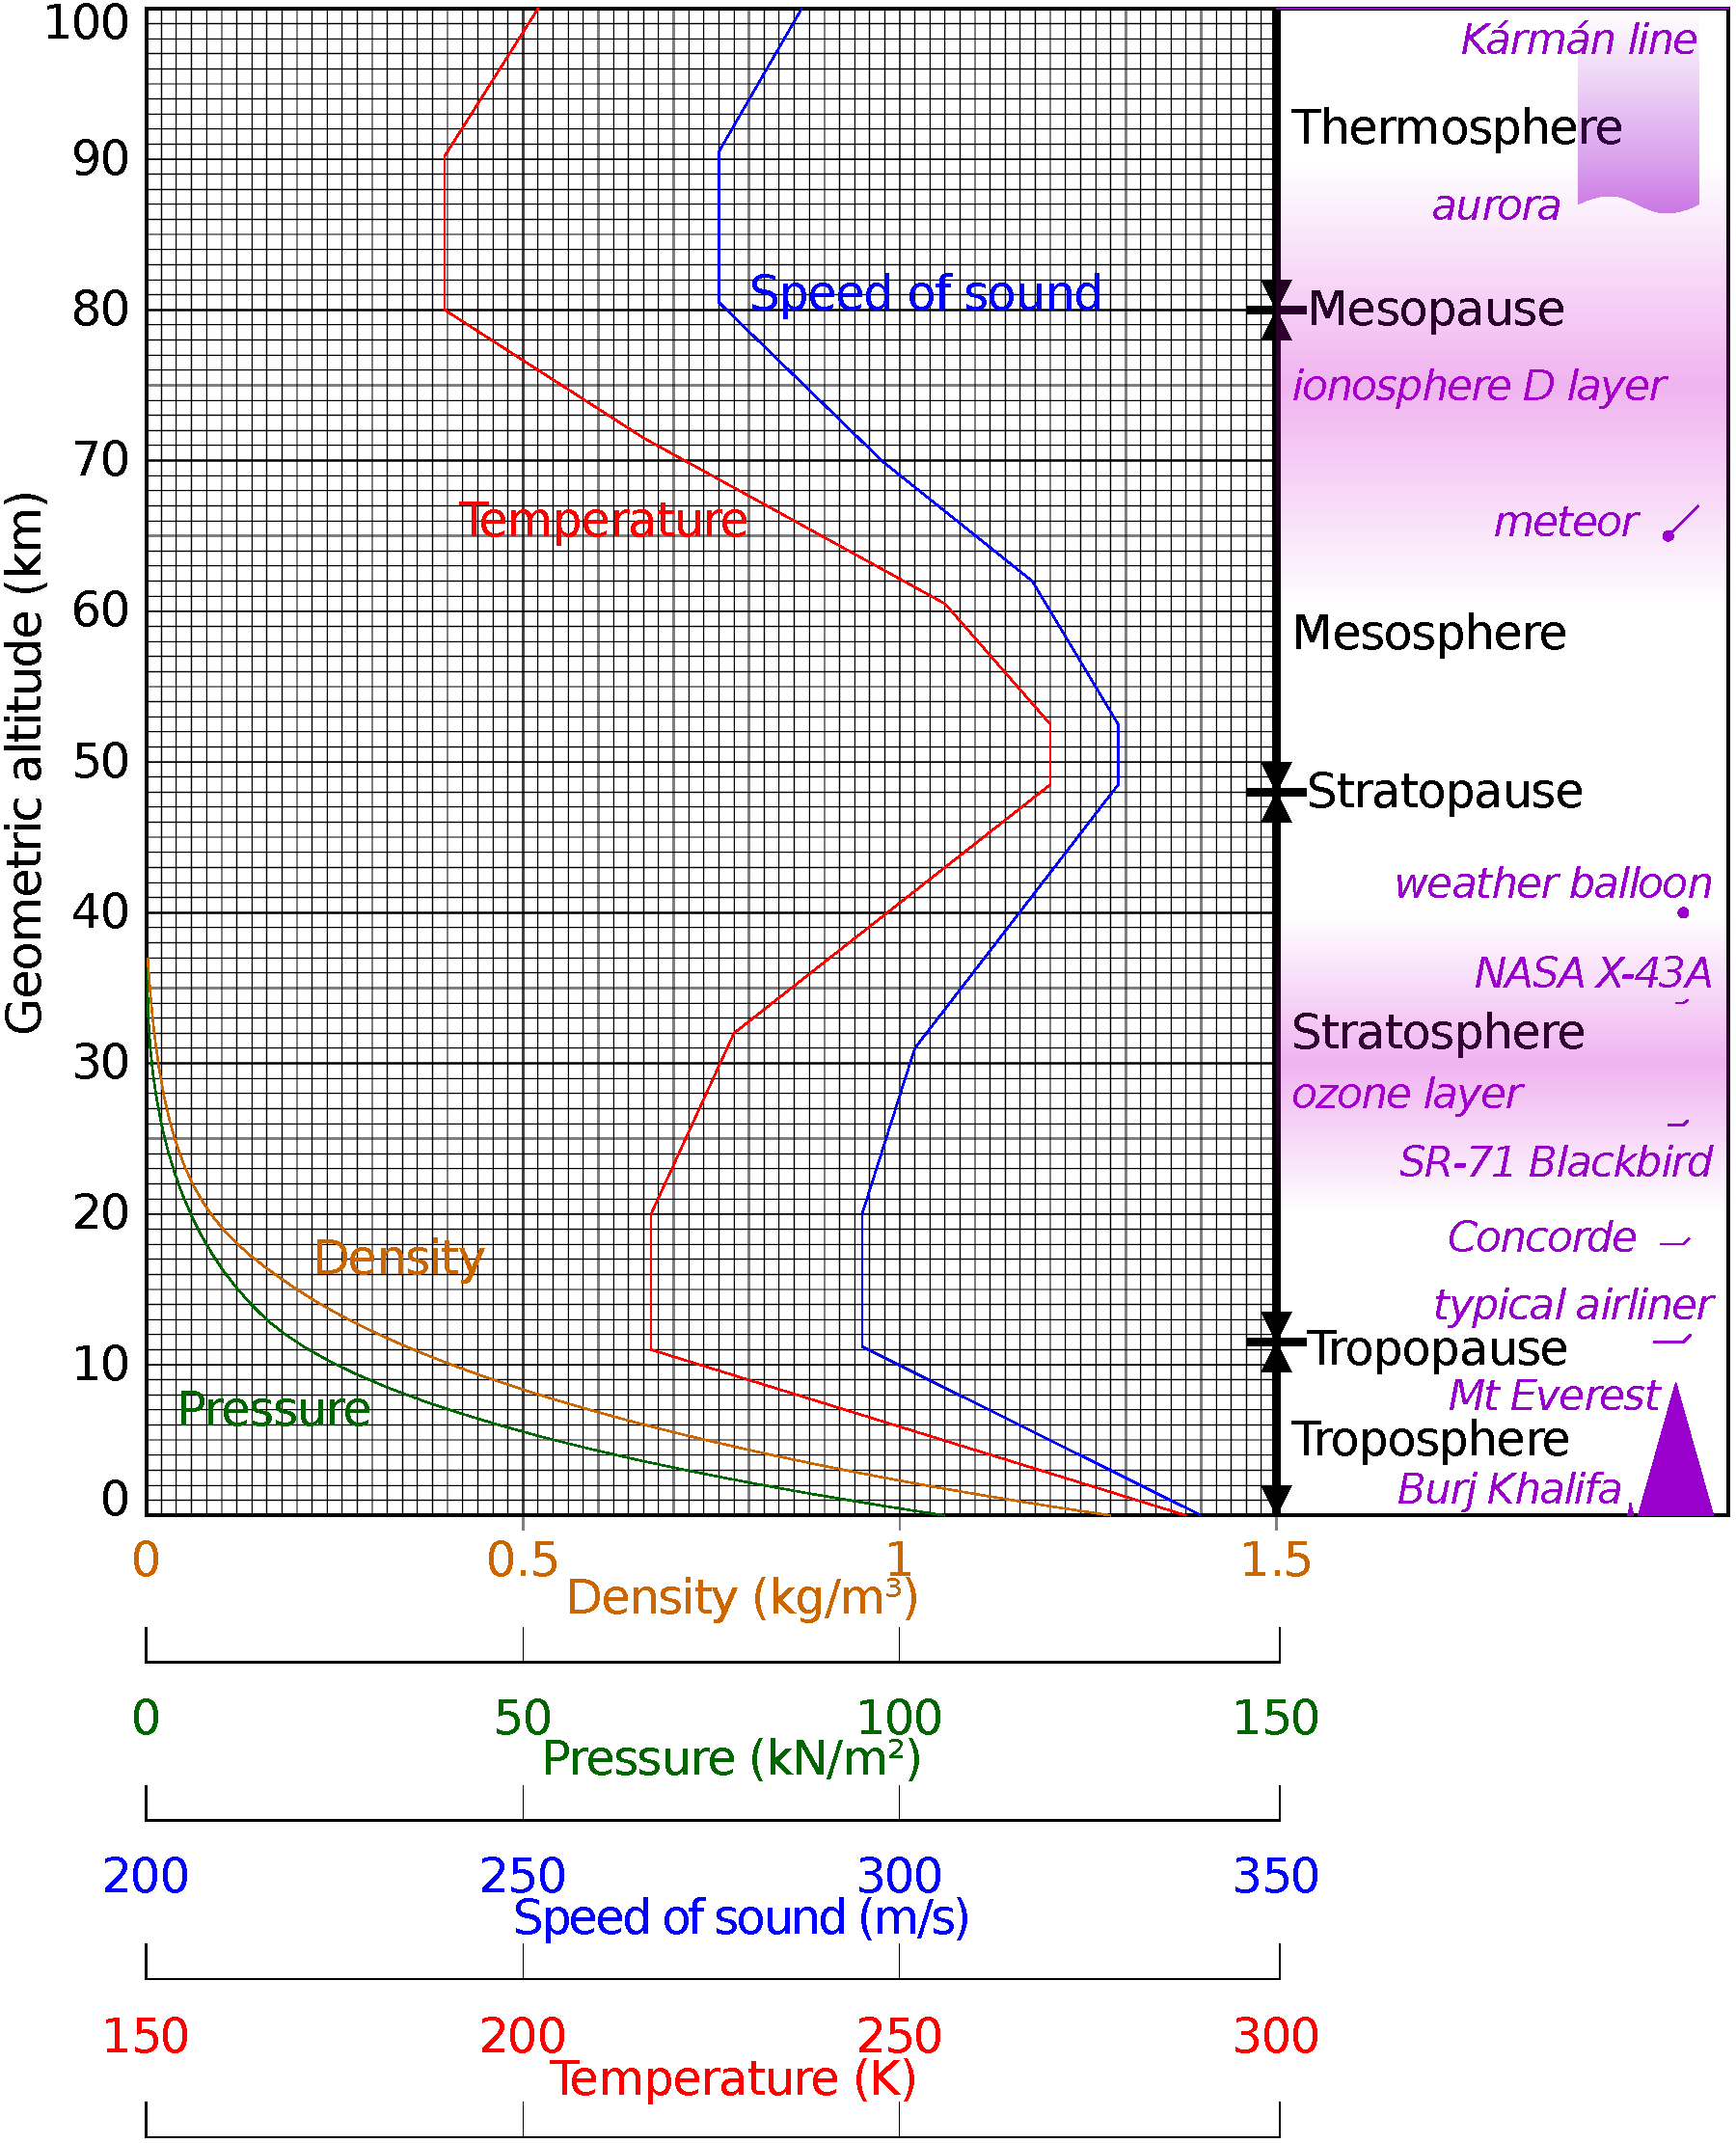
\includegraphics[width=0.6\linewidth]{chapter01/Comparison_US_standard_atmosphere_1962.pdf}
    \caption{%
        Comparaison des variables atmosphériques selon l'atmosphère standard définie par
        l'\textit{US standard atmosphere} de 1962.
        Source:
        \href{https://commons.wikimedia.org/wiki/File:Comparison_US_standard_atmosphere_1962.svg}{wikicommons},
        par \href{https://commons.wikimedia.org/wiki/User:Cmglee}{Cmglee}, CC-BY-SA.
    }%
    \label{fig:chapter01/Comparison_US_standard_atmosphere_1962}
\end{figure}

\subsubsection{La couche limite atmosphérique}%
\label{sub:la_couche_limite_atmospherique}

À l'intérieur de cette fine couche d'environ \SI{600}{km}, seule la troposphère,
c'est-à-dire les 13 premiers kilomètres, nous est directement familière. C'est en effet
dans la troposphère que les phénomènes météorologiques auxquels nous sommes habitués s'y
déroulent : nuage, vent, pluie, etc. Alors que l'atmosphère paraît immense, il est
important de noter la faible hauteur de cette couche.

La partie de la troposphère directement impactée par les effets de la surface terrestre
(friction, réchauffement, turbulence) est appelée la couche limite atmosphérique (CLA, ou
\textit{atmospheric boundary layer (ABL))}. Cette couche variant de quelques dizaines à centaines
de mètres selon les lieux et périodes de la journée, a une dynamique rapide et
convective. Notamment intéressant pour cette thèse, cela a pour conséquence que les
émissions de surface anthropiques ou naturelles, et notamment les polluants, sont
redistribuées sur l'intégralité de cette hauteur.

Durant la nuit, la hauteur de la CLA est faible du fait de l'affaiblissement du
gradient thermique vertical lié à l'absence de réchauffement radiatif du sol (voir
Figure~\ref{fig:chapter01/Atmospheric_boundary_layer}) et la mise en place de la couche de
surface après le coucher du soleil. À l'aube, la surface se réchauffe et la
convection se met en place, rendant la CLA beaucoup plus homogène et diluant gaz et
particules dans un plus gros volume d'air. Les composés ne traversent cependant que
rarement la couche d'inversion thermique, limite entre la CLA et la troposphère libre.
Ainsi, après le coucher du soleil, on observe fréquemment une couche résiduelle au milieu de
la CLA qui ``capture'' les composés d'une journée à une autre.

Il est à noter que des couches d'inversions thermiques à plus basse altitude peuvent se
mettre en place, notamment dans les vallées alpines. Pour un flux d'émission
constant, cela entraîne donc une accumulation forte des composés chimiques dans un volume
très restreint, augmentant mécaniquement les concentrations.
\cite{allardQualite2018} a ainsi pu montrer que le gradient thermique est l'un des
facteurs explicatifs le plus important pour la compréhension des concentrations en
vallées alpines.
%Notamment, certains jours à Passy, France, un facteur de concentration de 700 était présent entre 

\begin{figure}[h]
    \centering
    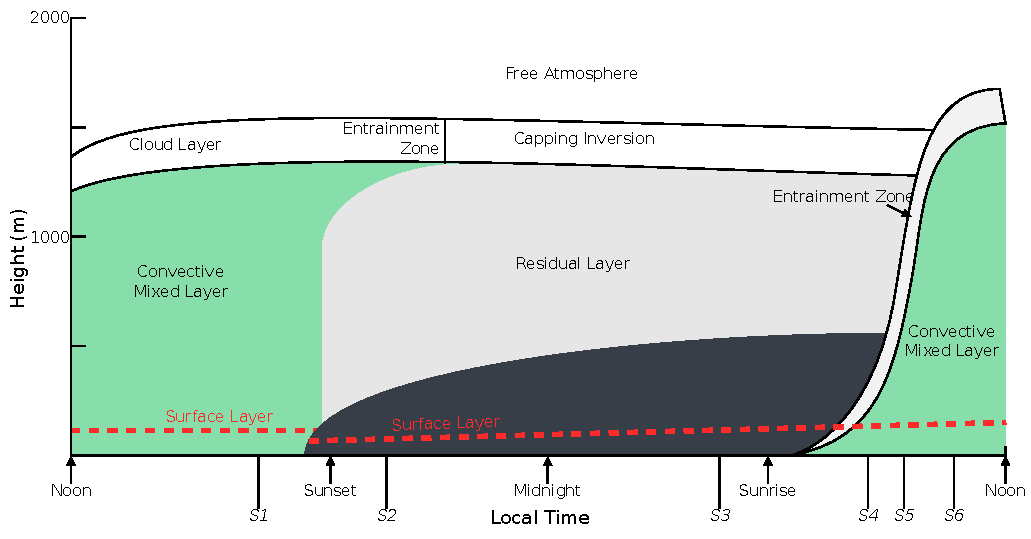
\includegraphics[width=0.8\linewidth]{chapter01/Atmospheric_boundary_layer.pdf}
    \caption{Évolution journalière schématique de la couche limite atmosphérique.
        Credit: By
        \href{https://commons.wikimedia.org/w/index.php?curid=18862904}{NikNaks} - Own
        work based on:
        \url{http://ars.sciencedirect.com/content/image/1-s2.0-S0360128504000371-gr4.jpg}.
        See also: \url{http://www.archaeocosmology.org/eng/tropospherelayers.htm}., CC
        BY-SA 3.0
    }%
    \label{fig:chapter01/Atmospheric_boundary_layer}
\end{figure}


\section{Les aérosols atmosphériques}%
\label{sec:les_aerosols_atmospheriques}

\subsection{Qu'est-ce qu'un aérosol?}%
\label{sub:quest-ce-quun-aerosol}

L'air que nous respirons est constitué majoritairement de gaz (\ce{N2}, \ce{O2}…) mais
également de particules solides ou liquides en suspension dans l'air. Très
légères et de tailles de l'ordre du nanomètre à quelques dizaines de micromètres,
ces particules sont communément appelées particules fines, ou \textit{particulate matter} (PM).

À titre de comparaison, cela reviendrait à grouper dans une même catégorie une marche de
\SI{100}{m} pour aller chercher son pain à un voyage de \SI{10000}{km}.
Ainsi, cette nomenclature ``PM'' regroupe nécessairement des objets aux caractéristiques
très diverses, comme le montre la Figure~\ref{fig:aerosolDistribution}. Selon
que l'on observe les PM en s'intéressant à leur nombre, surface ou volume, l'importance
relative des classes de taille change complètement.

\begin{figure}[ht]
    \centering
    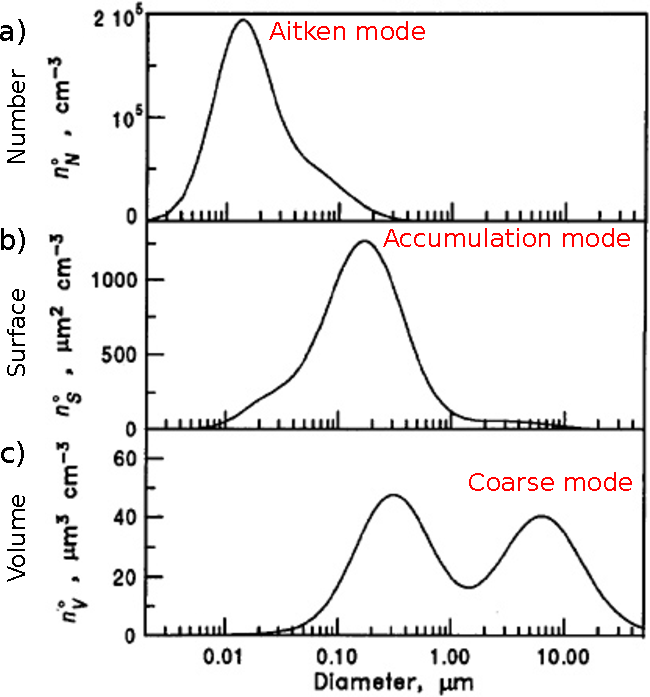
\includegraphics[width=0.5\textwidth]{aerosolDistribution.pdf}
    \caption{Distribution \textbf{(a)} en nombre, \textbf{(b)} surface, et
        \textbf{(c)} volume, pour un ensemble typique de distribution trimodale
        d'aérosols. Figure adaptée du livre de~\cite{seinfieldAtmospheric1998}.}
    \label{fig:aerosolDistribution}
\end{figure}

Ces différentes classes de taille (appelées modes) sont dues à différents procédés à
l'origine de leurs présences dans l'air. Le mode le plus fin et prépondérant en nombre,
dit d'Aikten, correspond à la nucléation à partir de composés gazeux ou de sources de
combustion.  Par coagulations successives et transformations dans les nuages, des
particules plus grosses se forment (mode d'accumulation).  Enfin se forme le mode grossier
alimenté par diverses autres sources comme la remise en suspension de poussières ou sable
par le vent, les pollens, les activités humaines, parmi d'autres, comme nous le verrons
plus loin.

La nomenclature des aérosols est ainsi historiquement fondée sur leur taille:
\begin{itemize}
    \item \PMdix, dont le diamètre aérodynamique est inférieur ou égal à \SI{10}{\um} (petit
        grain de sable, pollens…)
    \item \PMdc, dont le diamètre aérodynamique est inférieur ou égal à \SI{2.5}{\um}
        (suie, fumée…)
    \item \PMun, parfois appelées particules ultrafines (UFP), dont le diamètre
        aérodynamique est inférieur ou égal à \SI{1}{\um} (coagulation et condensation de
        vapeur…)
\end{itemize}


Ces catégories très diverses présentent ainsi des formes variées, comme illustré par les
clichés de microscopies électroniques présentés figure~\ref{fig:micrography}. On retrouve
des particules sphériques de petites tailles, des formes plus géométriques issues de
processus de cristallisation comme le sel marin, etc.

\begin{figure}[ht]
    \centering
    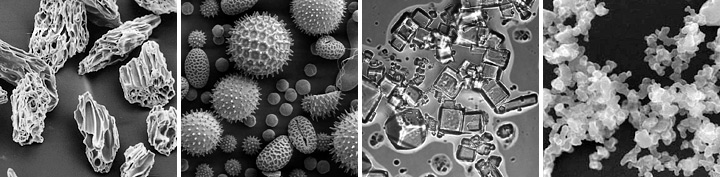
\includegraphics[width=1.0\textwidth]{aerosol_micrographs.jpg}
    \caption{Image au microscope électronique à balayage, à des échelles différentes,
        illustrant la diversité de forme des aérosols.
        De gauche à droite : cendre volcanique, pollen, sel de mer et suie. Micrographies de
        l'USGS, UMBC (Chere Petty) et de l'Arizona State University (Peter Buseck). 
        Crédit : NASA earthobservatory \url{https://earthobservatory.nasa.gov/Features/Aerosols/}.
    }
    \label{fig:micrography}
\end{figure}

\subsection{Composition chimique}%
\label{ssub:composition_chimique}

Les espèces chimiques constitutives des PM sont regroupées en différents groupes. La
figure~\ref{fig:chapter01/composition_chimique} présente les gammes de concentrations
observées à travers le monde pour différentes typologies de sites de prélèvement.
On y trouve divers ions issus de la condensation de la phase gazeuse : nitrate \NOt{} formé à
partir des \ce{NO_x}; ammonium \NHq{} formé à partir de \NHt; sulfate \SOq{} formé par
condensation et réaction chimique du \ce{SO2}.
Une part importante de la masse provient de la matière carbonée, notée ici
carbone organique (ou \textit{organic carbon} OC). Ce terme regroupe un nombre extrêmement
important d'espèces chimiques comportant une chaîne carbonée, de l'oxygène et
de l'azote. On y trouve par exemple la cellulose ou autres sucres issus de sa
dégradation par combustion (lévoglucosan, mannosan, galactosan), des ``polyols'' (arabitol,
mannitol, etc) émis par les bactéries ou champignons~\autocite{samakePolyols2019}, ou encore
d'autres familles de molécules comme les alcanes, hopanes, composés aromatiques
polycycliques ou pesticides. Cette matière carbonée est souvent nommée matière
organique (MO, ou \textit{organic matter} OM) afin de prendre en compte la masse du
carbone et celles des autres atomes (oxygène, azote…). Le facteur correctif entre OC et OM
varie entre 1.2 et 2.3 suivant les lieux de prélèvement.
Mais le carbone est également présent sous forme plus ``pure'' (i.e. avec très peu
d'oxygène ou autres atomes).
On parle alors de carbone élémentaire (\textit{elementary carbon} EC) lorsqu'il est mesuré
par méthode thermique, et de carbone noir (\textit{black carbon} BC) lorsqu'il est mesuré
par méthode optique. Cette distinction EC ou BC provient du fait qu'il existe un continuum
entre le carbone organique et le carbone élémentaire, et chacune des méthodes
d'observation implique un seuil différent de séparation entre ces deux catégories.
Pour finir, d'autres ions sont également présents, comme le sodium \ce{Na^+}, le chlore
\ce{Cl-}, le magnésium \ce{Mg^2+}, etc. mais également de nombreux éléments métalliques
comme le cuivre \ce{Cu}, l'aluminium \ce{Al}, le titane \ce{Ti}, le calcium \ce{Ca}, le fer
\ce{Fe}, etc.

La composition chimique d'un aérosol dépend de ses sources d'émissions
(voir~\ref{sub:profil_chimique_des_sources_d_émissions_courantes}) mais également des
différents processus bio-physico-chimiques présents dans l'atmosphère. Sous l'effet des
radiations solaires, de la capacité oxydante de l'atmosphère ou des micro-organismes
vivant dans l'air, la composition chimique des aérosols évolue au cours de leur vie.
Lorsque les espèces chimiques constituant les aérosols sont identiques à celles émises par
les différentes sources d'émission, on parle d'\textit{aérosol primaire}. En revanche,
lorsque les aérosols ont subi différentes modifications et présentent de nouvelles espèces
chimiques, on parle d'\textit{aérosol secondaire}.

Cette sensibilité aux sources d'émission explique en partie la variabilité observée pour la
composition chimique et sa sensibilité à la typologie du site d'étude. Par exemple, les
sites marins présentent davantage de sels marins, les sites proches des déserts de sable
ont davantage de poussières minérales, les sites urbains ont plus de marqueurs de
combustions (EC), etc.

\begin{figure}[ht]
    \centering
    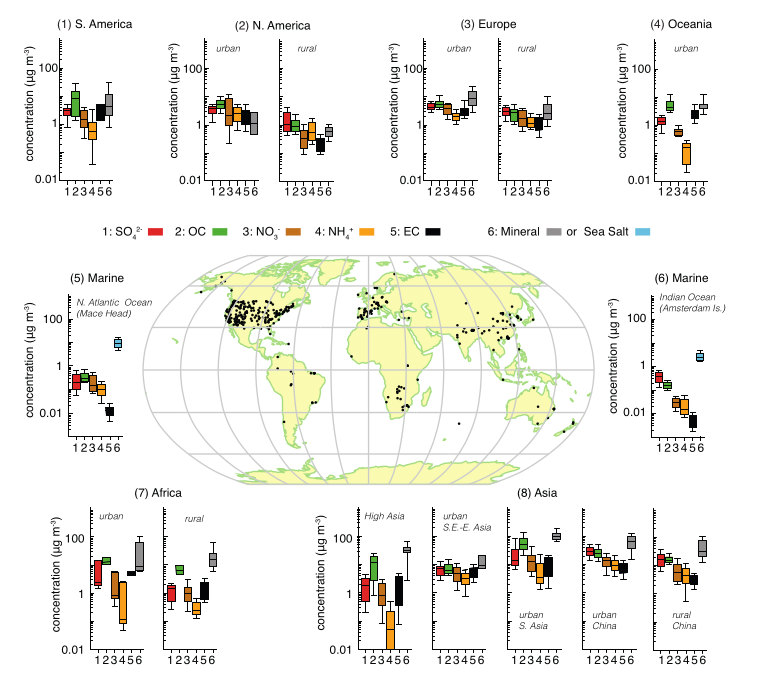
\includegraphics[width=1.0\linewidth]{chapter01/composition_chimique.png}
    \caption{Composition chimique majeure de la masse des \PMdix{} pour différentes
        typologies de sites de prélèvement. Crédit: \cite[figure 7.13]{boucherClouds2013},
        agrégeant 113 études sur au moins une année de prélèvement, entre 1993 et 2012.}%
    \label{fig:chapter01/composition_chimique}
\end{figure}

\subsection{Impacts des aérosols sur l'écosystème terrestre}%
\label{sub:impacts_des_aérosols_sur_l_écosystème_terrestre}

\subsubsection{Impacts climatiques}%
\label{ssub:impacts_climatiques}

Les aérosols sont des éléments essentiels de la machine climatique terrestre de par leur
interaction avec le rayonnement solaire et donc leur impact sur le bilan radiatif de la
Terre. Ils sont également essentiels de par leur interaction très forte avec la dynamique
des nuages, au point que les rapports du GIEC traitent dans le même chapitre les nuages et
les aérosols.

\paragraph{Impact radiatif}%
\label{par:impact_radiatif}

De par leur faible taille, les aérosols diffusent le rayonnement incident. Ils agissent
donc comme ``bouclier thermique'', ré-émettant une partie du flux solaire entrant dans
l'espace, conduisant ainsi à un refroidissement de l'atmosphère.  Cependant, les aérosols
absorbent aussi une partie du rayonnement incident, ce qui augmente l'agitation thermique
et donc conduit à un réchauffement du climat.  Ces deux effets antagonistes agissent de
concert à différentes altitudes de l'atmosphère et dépendent de la composition chimique
des aérosols.  Enfin, le dépôt des aérosols et notamment du \textit{black carbone} sur la
neige ou les glaces des banquises induit un effet bien connu de rétroaction positive. Le
carbone diminue l'albédo et absorbe le rayonnement normalement réémis par les surfaces
blanches, augmente donc localement la température et fait fondre la glace, découvrant
ainsi des surfaces plus sombres (roche ou océan) absorbant davantage de rayonnement,
conduisant à un réchauffement accru, et ainsi de suite.

\paragraph{Impacts sur la dynamique des nuages}%
\label{par:noyaux_de_condensation_des_nuages}

Les aérosols, grâce à leurs tailles et leurs ions, permettent en revanche de baisser
l'énergie d'activation nécessaire à l'agrégation de la vapeur d'eau sous forme liquide en
gouttelettes, puis gouttes, facilitant l'apparition des nuages. Ainsi, les aérosols agissent
comme noyaux de condensation des nuages (CCN pour \textit{cloud condensation nuclei}).
Certes, les nuages empêchent les infrarouges terrestres de repartir vers l'espace, mais
présentent également un albédo élevé renvoyant une grande partie du rayonnement à courte
longueur d'onde du Soleil vers l'espace. L'effet observé est donc un refroidissement de
l'atmosphère.
Aussi, pour une même quantité d'eau, le nombre de CCN disponibles conditionne la taille des
gouttelettes des nuages donc la taille de ceux-ci, leur durée de vie et probabilité de se
transformer en nuage précipitant.

\paragraph{Impacts sur le dérèglement climatique en cours}%
\label{par:impacts_sur_le_dereglement_climatique_en_cours}

Du fait de ces différents aspects antagonistes, très brièvement exprimés ci-dessus,
l'impact total des aérosols sur le climat n'est connu qu'avec une incertitude élevée. 

La contribution des aérosols à la différence du forçage radiatif entre 1750 et 2011 s'estime entre
\SIrange[range-phrase=~et~]{-0.77}{0.23}{\W\per\m\squared} (pour un forcage total actuel
de \SI{2.29}{\W\m\squared}), avec un forçage négatif pour
les poussières minérales, le sulfate, nitrate et carbone organique, mais positif pour le
carbone suie.  Quant à leur rôle sur la dynamique des nuages, il s'estime entre
\SIrange[range-phrase=~et~]{-1.33}{-0.06}{\W\per\m\squared}, mais présente des
incertitudes plus élevées du fait de la complexité à prendre en compte ces phénomènes dans
les modèles de climat. C'est actuellement le forçage radiatif le moins bien connu de la
machine climatique Terrestre.

\subsubsection{Impacts environnementaux}%
\label{ssub:impacts_environnementaux}

La durée de vie des aérosols dans l'atmosphère entre leur émission et leur déposition est
de plusieurs jours pour la majorité d'entre eux. Dans ce délai, la circulation atmosphérique les déplace sur des
distances pouvant atteindre plusieurs milliers de kilomètres. Il n'est pas rare par exemple en
Europe d'avoir des épisodes de dépôts de sable provenant du désert saharien. Ce
déplacement longue distance d'aérosols est même un des mécanismes clef de certains
\textit{bloom}
de phytoplancton, en apportant d'importantes quantités de nutriments à la surface de l'océan 
(métaux et phosphate notamment).
Autre exemple marquant, le nitrate, élément limitant de la croissance des
plantes en prairie d'altitude, est apporté en partie par
déposition de nitrate d'ammonium particulaire provenant du transport longue
distance~\autocite{bourgeoisFoliar2019}.

Plus spectaculaire, les cendres volcaniques relarguées dans l'atmosphère suite à de
violentes éruptions, en plus de leur impact climatique potentiel, peuvent occasionner des
pluies acides du fait de la présence en quantité de sulfate dans ces cendres.

Ces phénomènes présentent à quel point les aérosols et leur composition chimique variée
impactent directement de nombreux écosystèmes terrestres, et ce, qu'ils proviennent de sources
anthropiques comme c'est le cas pour le nitrate, ou bien de sources naturelles.

\subsection{Impacts sanitaires}%
\label{sub:impacts_sanitaires}

L'impact sanitaire des aérosols sur la population humaine a commencé à être
un sujet de recherche suite à l'industrialisation et aux épisodes de ``smog'' causant la
mort de nombreuses personnes à Engis (Meuse, Belgique) en 1930, Donora (Pennsilvanie, USA)
en 1948 ou encore le plus connu ``Great smog of London'', en 1952. Durant ces épisodes de
pollutions, il est important de noter que la sur-mortalité due à l'exposition aiguë
durant l'épisode est très importante (jusqu'à 3 fois supérieure à la normale
pour le smog de Londres), mais que la surmortalité persiste dans les mois qui suivent
--pendant près d'un an pour le smog de Londres-- alors même que les niveaux de pollution
étaient revenus à leurs états antérieur à décembre 1952 \autocite{bellReassessment2001}.  Ces
épisodes de pollution intenses marquent le début de la prise de conscience par la
population de la problématique de la pollution de l'air et ont conduit à la première
législation anglaise en matière de qualité de l'air en 1956 avec le \textit{Clean Air
Act}. Aussi, des programmes de mesures de la qualité de l'air pour différents polluants
ont émergé et les actions mises en œuvre au niveau national et international ont permis
en Europe une amélioration très sensible de la qualité de l'air
(Figure~\ref{fig:chapter01/tendance_polluants}).

\begin{figure}[ht]
    \centering
    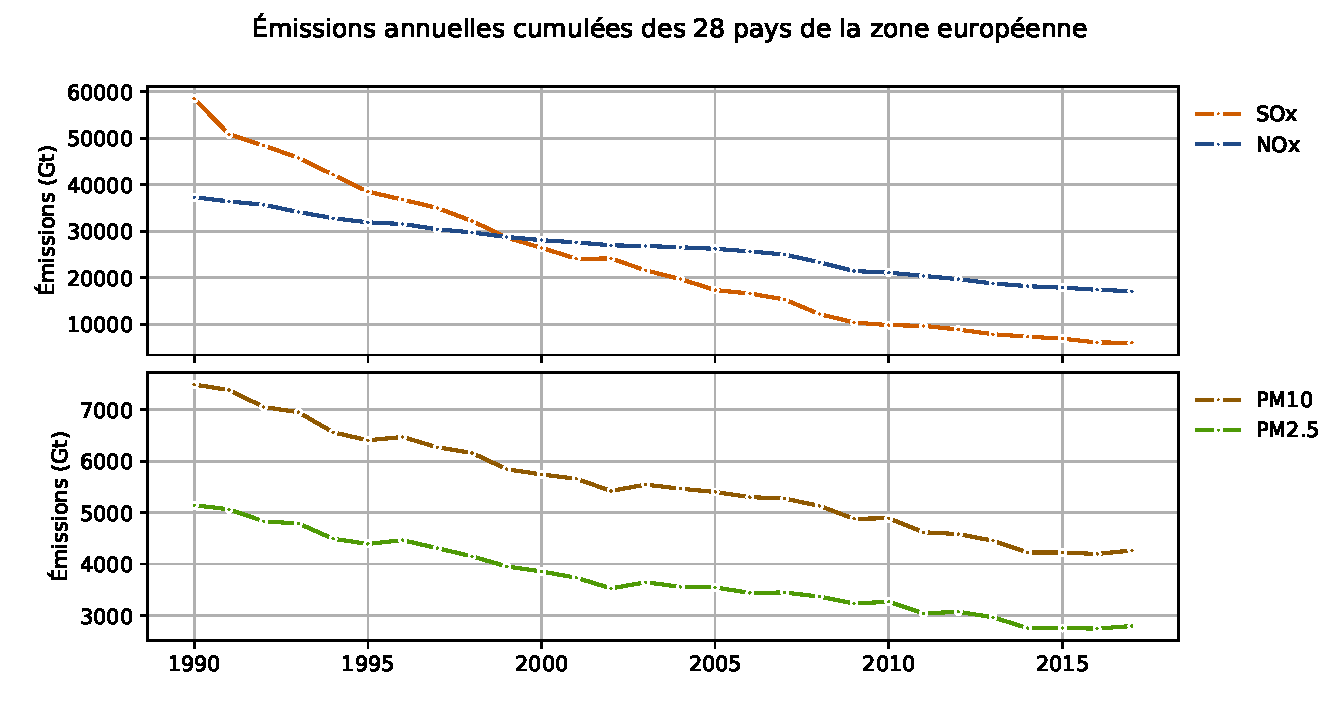
\includegraphics[width=0.9\linewidth]{chapter01/tendance_polluants.pdf}
    \caption{Évolution temporelle des émissions cumulées des 28 pays de la zone européenne
    depuis 1990, indiquant une prise de conscience et une diminution des émissions de
    différents polluants gazeux (\ce{SO_x} et \ce{NO_x}) et particulaires (\PMdix{} et \PMdc). Données
issues de \textit{National emissions reported to the Convention on Long-range
Transboundary Air Pollution (LRTAP Convention)}, ©European Environment Agency (EEA).}%
\label{fig:chapter01/tendance_polluants}
\end{figure}


Cependant, la qualité de l'air (incluant les aérosols, mais également les
composés gazeux comme les \ce{NO_x} ou l'ozone) demeure actuellement la 5\ieme{} cause de
mortalité dans le monde, représente un décés sur dix et est catégorisée ``cancérogène
certain'' par le CIRC depuis 2013. En Europe, pour l'année 2013, c'est
ainsi \num{800000} personnes qui sont décédées des suites de maladies cardiovasculaires,
cancer, pneumonie… directement attribuables à la qualité de l'air
\autocite{worldhealthorganizationAmbient2016}. Récemment, \cite{lelieveldLoss2020}
estiment qu'en moyenne et à travers le monde, c'est \num{2.9} ans de vie perdue par personne
qui sont imputables à la pollution de l'air, dont \num{1.7} ans ``évitables'' car provenant
directement de sources anthropiques.

En termes de bilan financier, la banque mondiale en collaboration avec l'Institute for
Health Metrics and Evaluation (IHME) de l'université de Washington estimait que le coût
associé aux décés prématurés de la seule année 2013 s'évaluait à plus de \$5.11 trillions
de dollar dans le monde~\autocite{worldbankCost2016}.

Afin de limiter cet impact sanitaire, de nombreux pays ont défini des seuils de
concentrations de différents composés (voir Tableau~\ref{tab:seuil_PM} pour les PM).
Seulement ces seuils sont différents d'une institution à une autre. Par exemple, entre
2015 et 2017, le seuil de concentration journalière recommandé pour les \PMdix{} par
l'union européenne (\SI{50}{\ugm} en moyenne journalière) était dépassé pour 13 à
19~\% de la population européenne, mais cette proportion augmente entre 42 et 62~\% si
l'on prend en compte le seuil recommandé de l'OMS de \SI{20}{\ugm} en moyenne
annuelle~\autocite{europeanenvironmentagencyAir2019}.  De plus, il est à noter qu'il
n'existe pas de seuil à partir duquel l'exposition aux PM est inoffensive.

\begin{table}[ht]
    \begin{ThreePartTable}
        \centering
        \caption{Seuils de concentration de PM recommandés par différents organismes.}
        \label{tab:seuil_PM}
        \begin{tabular}{ccSc}
            \toprule
            Organisme       & Polluant & {Concentration (\si{\ugm})} & Période \\
            \midrule
            OMS\tnote{a}    & \PMdc  & 10 & moyenne annuelle       \\
            OMS\tnote{a}    & \PMdc  & 25 & moyenne sur \SI{24}{h} \\
            OMS\tnote{a}    & \PMdix & 20 & moyenne annuelle       \\
            OMS\tnote{a}    & \PMdix & 50 & moyenne sur \SI{24}{h} \\
            Europe\tnote{b} & \PMdc  & 25 & moyenne annuelle       \\
            Europe\tnote{b} & \PMdc  & 20 & moyenne sur 3 ans      \\
            Europe\tnote{b} & \PMdix & 40 & moyenne annuelle       \\
            Europe\tnote{b} & \PMdix & 50 & moyenne sur \SI{24}{h} \\
            France\tnote{c} & \PMdc  & 25 & moyenne annuelle       \\
            France\tnote{c} & \PMdix & 50 & moyenne sur \SI{24}{h} (\SI{<35}{jour\per an}) \\
            France\tnote{c} & \PMdix & 40 & moyenne annuelle \\
            \bottomrule
        \end{tabular}
        \begin{tablenotes}
        \item[a] OMS air quality guideline \cite{worldhealthorganizationWHO2006}
        \item[b] Directive 2008/50/EC \cite{officialjournaloftheeuropeanunionDirective2008}
        \end{tablenotes}
    \end{ThreePartTable}
\end{table}

\section{Détermination des sources d'émission des PM}%
\label{sec:source_apportionment_of_pm}

Comme nous l'avons vu, les sources d'aérosols sont très diverses.
Afin d'avoir un impact sur les concentrations de polluants via des
réglementations, il est primordial de
retracer leur provenance. Plusieurs techniques d'analyses existent, qu'elles soient purement
physiques ou géochimiques.

\subsection{Modèle d'attribution des sources}%
\label{sec:source_apportionment_model}

Afin d'estimer la contribution de chaque source de PM en un point donné, il est possible
d'utiliser deux grandes familles de modèles d'attribution des sources (\textit{source
apportionment} (SA)). La première est fondée sur notre connaissance des
émissions et de la météorologie et calcule les réactions physico-chimiques depuis les
sources jusqu'au lieu d'étude (modèle dit de chimie-transport (\textit{chemical transport
model} CTM) alors que la deuxième s'évertue à mesurer en un point donné
la chimie des PM et par traitement statistique, attribue à différentes sources ou
``facteurs'' leurs contributions aux concentrations observées (modèle dit récepteur
(\textit{receptor model} RM)).

\subsubsection{Modèle déterministe de chimie-transport}%
\label{ssub:modele_deterministe_de_chimietransport}

\paragraph{Présentation}%
\label{par:presentation}

Les modèles déterministes s'appuient sur l'inventaire des sources d'émissions sur la
région étudiée. Ces cadastres d'émissions sont regroupés en catégories \textit{Selected
Nomenclature for reporting of Air Pollutants} (SNAP) représentant chacune un secteur
d'activité : Énergie, Procédés industriels, Agriculture, Déchets, Autres et enfin
Naturelle.
Chacune de ces catégories possédant évidemment des sous-catégories raffinant la
classification (par exemple, les émissions de l'aviation civile des avions de plus de \SI{100}{m} de
long se retrouvent dans le SNAP 080503 (ou \textit{Nomenclature For Reporting} (NFR)
1.3.A.c) autrement dit Énergie - Combustion - Aviation - Aviation civile de plus de
\SI{100}{m})~\autocite{europeanenvironmentagencyEMEP2019}.
À chacune de ces SNAP est associé un profil d'émission (\ce{O3}, \ce{SO2}, \ce{NO_x}, \ce{NH3}, \PMdix, \PMdc,
VOC principalement), obtenu soit par mesure directe, soit par calcul.

Vient ensuite un inventaire de ces sources d'émissions sous forme de cadastre géographique
et temporel. Notamment la \textit{Convention on Long-Range Transboundary Air
Pollution} (LRTAP) implémentée par l'\textit{European Monitoring and Evaluation Program}
(EMEP) sous l'égide de \textit{United Nations Economic Commission for Europe} (UNECE)
prévoit que les différentes parties prenantes à cette convention (i.e. les pays membres)
présentent un rapport de leurs émissions régulièrement à l'EMEP.

Il est alors possible de construire des modèles déterministes de dispersion et de
réaction des polluants, en couplant un modèle de diffusion résolvant les équations de la
physique de l'atmosphère (Navier-Stoke, turbulence, rayonnement, etc) avec un modèle
physico-chimique faisant évoluer les composés gazeux et particulaires, incluant leurs
émissions, dépôts, interaction physico-chimique, etc. Pour n'en citer que quelques-uns : 
Community Multi-scale Air Quality (CMAQ)\footnote{CMAQ: \url{https://www.epa.gov/cmaq}},
Comprehensive Air Quality Model with Extensions (CAMx)\footnote{CMAx : \url{http://www.camx.com/}},
WRF-Chem\footnote{WRF-chem : \url{https://www2.acom.ucar.edu/wrf-chem}},
Chimère,
LOTOS-EUROS...

La raison de la pluralité de ces modèles provient des différentes paramétrisations
possibles des équations physiques, mais également des choix conceptuels de recherche.

\paragraph{Estimation de la contribution des sources d'émissions par CTM}%
\label{par:source_apportionment}

Concernant l'attribution des sources, il est possible d'utiliser deux techniques au sein
des CTM:

\begin{enumerate}
    \item Faire une première simulation incluant toutes les sources d'émissions (référence
        ou témoin), puis une deuxième simulation avec une source d'émission en moins. La
        différence reflétant l'impact de la source supprimée sur les concentrations
        ambiantes (technique dite de force-brute);
    \item Garder en mémoire la provenance de chacune des espèces chimiques lors des
        schémas réactionnels (technique dite de \textit{source labelling} ou \textit{tagged species}).
\end{enumerate}

Seulement, du fait des nombreux processus non linéaires, la suppression d'une source
d'émission aura des répercussions beaucoup plus complexes que la simple diminution des
concentrations propres à cette source (par exemple, des NOx pourraient ne pas passer en
phase particulaire du fait d'un manque d'ammoniac, ou inversement). 
% TODO: élaborer ou supprimer cette partie
%La première technique correspond donc à se demander 
%\begin{quote}
%    Si les émissions de cette source sont diminuées ou supprimées, quels impacts cela va-t-il
%    avoir sur les concentrations finales ?
%\end{quote}
%alors que la deuxième répond à
%\begin{quote}
%    Dans la concentration ambiante de PM, à combien s'estime la contribution de cette source
%    d'émission ?
%\end{quote}
%Ce sont bien deux questions différentes avec leurs légitimités propres.
La seconde technique a commencé à être implémentée plus récemment dans certains
CTM~\autocite{wangDevelopment2009,wagstromDevelopment2008,kranenburgSource2013,brandtContribution2013}
et elle est détaillée dans le rapport de~\cite{mirceaEuropean2020}. Elle présente également
l'avantage de pouvoir tagguer non seulement les sources des espèces chimiques, mais
également leur provenance géographique, c'est-à-dire leur lieu d'émission.

\paragraph{Limitations}%
\label{par:limitations}

Cependant, l'utilisation des CTM présente certaines limites du fait de leur complexité.
Notamment, il semble illusoire de pouvoir un jour inclure toutes les réactions chimiques
possibles dans les modèles déterministes. Par exemple, les interactions aérosols/neige ou
même plus simplement les interactions aérosols/nuages et la chimie aqueuse qui s'y produit
ne sont pas encore complètement comprises ni bien représentées dans ces modèles.

Quand bien même ce serait le cas --car les modèles réactionnels sont de plus en plus
poussés--, 
ces modèles déterministes reposant sur une connaissance a priori la plus complète
possible, il faudrait alors avoir des inventaires d'émissions beaucoup plus complets et
précis temporellement, avec aucune certitude d'un oubli potentiel d'une source non prise
en compte. Ce sont par exemple, une industrie locale non-encore répertoriée, la sous-estimation de
la contribution d'un écosystème, une consommation de bois de chauffage individuel non
inventoriée, etc.
En plus de cette connaissances de la quantité des émissions, leurs distributions
temporelles et spatiale s'avère également compliquée. Notamment, la répartition annuelle
de la quantité de bois de chauffage totale peut s'avérer approximative selon les
paramétrisations des modèles et ne pas représenter la réalité des émissions.

Aussi, la limitation physique des modèles météorologiques se retrouvent dans les CTM. Il
est donc compliqué d'envisager, du fait du coût de calcul et de stockage, une simulation à
\SI{10}{\m} de résolution spatiale (ou moins), ce qui serait cependant nécessaire pour
appréhender correctement des phénomènes précis.
Notamment, les milieux complexes comme les vallées alpines demandent une résolution fine
du fait d'une topographie très variable et des sources d'émissions localisées.
\cite{bessagnetHigh2020} ont montré que l'augmentation de la résolution spatiale améliore
en partie les prédictions de ces modèles sur la vallée de l'Arve et Grenoble, mais un
biais négatif de l'ordre de \SI{10}{\ugm} pour les \PMdix{} demeure.
En dehors de ces travaux de recherches à fine échelle, les prévisions opérationelles
francçaise de PREV'AIR \parencite{rouilPrev2009} se font à résolution spatiale de l'ordre
de \SI{4}{\kilo\m} alors que la vallée de l'Arve ne fait qu'un kilomètre de large. De
fait, les prévisions ne pourront pas prendre en compte certains phénomènes très locaux.


\subsubsection{Modèles récepteurs}%
\label{ssub:model_recepteur}

À l'inverse des CTM, il est possible d'estimer les sources contribuant aux concentrations
ambiantes en un lieu donné sans la moindre information météorologique ou simulation
déterministe. Pour cela, il convient de faire des prélèvements sur le lieu d'étude,
d'analyser la chimie que l'on y trouve et retrouver à l'aide d'un modèle statistique
les différents profils de source et leurs contributions, ce qui peut se traduire en
particulier par l'équation d'équilibre des masses
\begin{align}
    \label{eq:mass_balance}
    X &= G \cdot F
\end{align}
où $X$ est la matrice de dimension $n\times m$ des observations, $G$ est la matrice des
contributions de taille $n\times p$ et $F$ la matrice des profils de taille $p \times n$,
avec $n$ le nombre d'échantillons, $m$ le nombre de variables chimiques mesurées et $p$ le
nombre de facteurs.
Un \textit{facteur} peut être une source d'émission (combustion de biomasse par exemple),
mais également regrouper des espèces chimiques provenant d'un même processus secondaire
(nitrate d'ammonium par exemple).
Il est courant d'exprimer $X$ en \si{\ugm}, $G$ en \si{\ugm} ou concentration
normalisée~\si{[-]} et $F$ en concentration relative \si{[-]}
(i.e.~\si{\micro\g\per\micro\g}) ou \si{\ugm}.

Si l'on mesure $X$, ce qui nous intéresse ici est de connaître $G$ ou $F$.
Si l'on admet que l'on connait a priori les profils d'émissions possibles, alors $F$ est
connue et l'on cherche à estimer $G$. Le modèle de déconvolution adapté est alors le
\textit{Chemical Mass Balance} (CMB). À l'opposé, on peut n'avoir aucune information a
priori à la fois sur les contributions et les profils d'émissions. On utilisera alors le
modèle de déconvolution \textit{Positive Matrix Factorization} (PMF).

Ces 2 types de modèles statistiques sont aux deux extrêmes d'un spectre de modèles de
déconvolution, depuis une information ``absolue'' des profils de sources à une absence
totale d'information sur ces mêmes profils.  Il existe cependant un continuum entre ces
deux pôles (voir Figure~\ref{fig:chapter01/source_apportionment_methods}), et de nombreux
modèles ont été développés et améliorés depuis la première étude de SA de
\cite{colucciAutomotive1965} utilisant la ``simple'' corrélation entre le \ce{CO} et
le plomb et benzo(a)pyrène.  Une revue détaillée et historique du fonctionnement de ces
différents modèles peut être retrouvée dans les articles de
\cite{henryHistory1997,vianaSource2008,belisCritical2013,hopkeReview2016}.

\begin{figure}[ht]
    \centering
    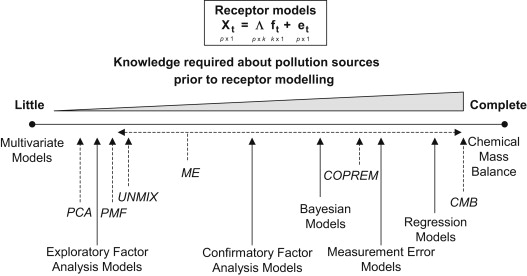
\includegraphics[width=0.7\linewidth]{chapter01/source_apportionment_methods.png}
    \caption{
        Connaissances a priori nécessaires pour les différents modèles de SA existant,
        depuis la simple analyse de facteur par ACP au modèle CMB. Crédit :
        \cite{vianaSource2008} adaptée de \cite{schauerCharacterization2006}
    }%
    \label{fig:chapter01/source_apportionment_methods}
\end{figure}

\subsubsection{Chemical mass balance CMB}%
\label{ssub:chemical_mass_balance_cmb}

Le principe du CMB est de déterminer la contribution $G$ d'un nombre de sources
aux profils chimiques $F$ prédéfinis aux concentrations ambiantes $X$. Il est donc
nécessaire de connaître les signatures chimiques des sources utilisées.

Afin d'utiliser le modèle CMB --mais également pour d'autres buts-- l'US EPA construit
depuis 1988 la base de données SPECIATE~\autocite{simonDevelopment2010}, répertoriant
différents profils d'émission, dont la 5\ieme{}
version a été publiée en 2019~\autocite{u.s.environmentalprotectionagencySPECIATE2019}.
Seulement, ces profils sont représentatifs des sources présentes aux États-Unis et sont
très certainement non transposables à d'autres régions du monde.
En Europe, il existe depuis 2016 une base de données similaire,
SPECIEUROPE~\autocite{pernigottiSPECIEUROPE2016}, compilant des mesures à l'émission et
les résultats d'autres types d'étude permettant d'estimer la signature chimique des
profils d'émission.

Cependant, des erreurs ou variabilités locales spécifiques au site récepteur sur ces
profils peuvent conduire à une estimation erronée des contributions finales des
différentes sources en utilisant le modèle CMB.
Aussi, il est nécessaire de choisir ou d'agréger certains des plus de 3000 profils de sources
différents répertoriés afin de restreindre à une valeur réaliste le nombre de sources
potentielles en un lieu donné.
Enfin, les processus secondaires sont mal pris en compte dans ce type de modèle. L'exemple typique
concerne l'aérosol inorganique secondaire sulfaté, représenté comme un mélange de sulfate
et d'ammonium. Or ce facteur secondaire est souvent associé en réalité à de la matière
organique ou d'autres espèces sulfatées.

\subsubsection{Positive Matrix Factor PMF}%
\label{ssub:pmf}

Un modèle beaucoup plus agnostique que le CMB pour résoudre l'équation de conservation de
la masse a été développé par~\cite{paateroPositive1994}. Dans cette formulation,
seule la matrice d'observation $X$ est connue, et les matrices de contribution $G$ et des
profils chimiques $F$ sont inconnues.

\paragraph{Formulation mathématique}%
\label{par:formulation_mathématique}

Le principe de la PMF provient initialement de la recherche sur le \textit{machine
learning}, et plus particulièrement de l'analyse factorielle appliquée au problème
bilinéaire $X=G\times F$. L'intérêt initial est de permettre une réduction
dimensionnelle sans perte d'information. Par exemple, en informatique, une image de $n$
par $m$ pixels forme une matrice $n\times m$ éléments. S'il est possible de retrouver
cette matrice par multiplication de 2 matrices $G$ ($n\times p$) et $F$ ($p \times m$),
alors la quantité d'information stockée dans $G$ et $F$ est $n
\times p + p \times m = p \times (n + m)$. Ainsi, tant que $p < \frac{n\times m}{n+m}$,
alors le nombre d'éléments de $G\times F$ est toujours inférieur au nombre d'éléments de
$X$, permettant un gain de mémoire de plus en plus important au fur et à mesure que $n$ et
$m$ augmentent.
Tout le problème réside en le fait de trouver la décomposition de $X$ en minimisant
l'erreur engendrée par cette simplification.

Aussi, on observe que la formulation $X = G\cdot F$ est similaire à celle de
la conservation de la masse (Eq.~\ref{eq:mass_balance}). Ce problème peut-être résolu par
analyse en composante principale (ACP), seulement, le résultat obtenu présente des
combinaisons linéaires (additive et soustractive) des différents composants. Cette possible
négativité des composants n'a pas de sens dans beaucoup de domaines physiques, y compris en
géochimie. \cite{paateroPositive1994} présentent donc une nouvelle méthode de
déconvolution, implémentant une contrainte de non-négativité, nommée \textit{Positive Matrix
Factorization} (PMF). 

La formulation est la suivante : étant donné une matrice d'observation $X$ de taille
$n\times m$, une matrice associée des incertitudes $U$ de taille $n \times m$ et un rang
$p$, alors 
\begin{align}
    \label{eq:pmf_formulation}
    X &= G \cdot F + E \\
    \forall i,k,j &, G_{ik}\geq 0 \text{ et } F_{kj}\geq 0\\
    Q &= \sum_{i=1}^n\sum_{j=1}^m E_{ij}^2/U_{ij}^2\label{eq:Qfunction}\\
    {Q, F} &= \argmin_{G,F} Q.
\end{align}

Différents algorithmes de résolution du système Eq.~\ref{eq:pmf_formulation} ont été développés.
L'implémentation initiale de~\cite{paateroLeast1997} a été améliorée pour pouvoir
ajouter des contraintes sur les matrices $G$ et $F$, notamment grâce au solveur
\textit{multi-linear engine} (ME-2) \autocite{paateroMultilinear1999}. En effet, il
n'existe pas de solution unique au problème Eq.~\ref{eq:pmf_formulation}, notamment, car le
système est invariant par rotation:
\begin{align}
    \label{eq:rotationalambiguity}
    X   &= G \cdot F + E \\
        &= (G \cdot T) \cdot (T^{-1} \cdot F) + E\\
        &= G' \cdot F' + E
\end{align}
et ainsi une infinité de solutions coexistent. 

\paragraph{Interprétabilité du modèle PMF}%
\label{par:interpretabilite_du_model_PMF}

L'avantage de la PMF réside en le fait que l'algorithme n'est pas fondé sur la
corrélation entre variables, comme c'est le cas de l'ACP, mais bien en la formation d'un
modèle additif linéaire de ce qui est observé.
\begin{quote}
    We shall not be satisfied in finding some correlations, we wish to form a quantitative
    model of what was observed! \autocite{paateroPositive1994}
\end{quote}

Il a été montré que la PMF est capable d'extraire des informations partielles cohérentes des
données là où l'ACP n'est qu'une représentation holistique~\autocite{leeLearning1999}. Par
exemple, appliquée à la reconnaissance d'image faciale, la PMF déconvolue les visages en
sous partie (bouche, sourcils, front, etc) alors que d'autres méthodes ``se contentent''
d'une approche globale de l'information et où seules les premières dimensions portent
l'information nécessaire à la reconstruction du signal (voir
figure~\ref{fig:chapter01/NMFvsPCA}).

\begin{figure}[ht]
    \centering
    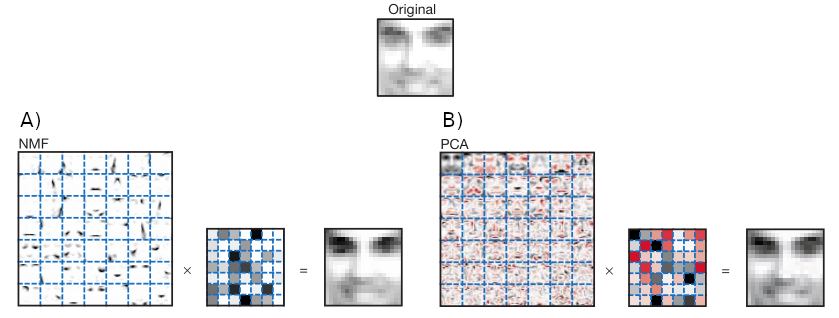
\includegraphics[width=1.0\linewidth]{chapter01/NMFvsPCA.png}
    \caption{Analyse factorielle par PMF (ou NMF pour \textit{non-negative matrix
    factorization}) et ACP d'une banque d'image de 2429 images en niveau de gris de 19
    pixels par 19 pixels. Les deux techniques essaient de reproduire l'image originale en
    fonction de leur apprentissage.
    \textbf{A)} Le rang de la PMF est $p=49$, correspondant aux 49
    représentations des $19\times19$ images à gauche, chacune étant un facteur de la
    matrice $F$, et leurs ``contributions'' respectivement identifiées par le carré de 7 par
    7 en niveau de gris, à droite.
    \textbf{B)} Analyse en composante principale, le carré de gauche représentant les 49
    vecteurs propres et celui de droite les 49 valeurs propres.
    Les échelles de couleurs sont : rouges pour les coefficients négatifs, noirs pour les
    coefficients positifs.
    Figure adaptée de \cite{leeLearning1999}}%
    \label{fig:chapter01/NMFvsPCA}
\end{figure}

\paragraph{Applicabilité en science de l'atmosphère}%
\label{par:applicabilité_en_science_de_l_atmosphère}

Dans le cas qui nous intéresse ici, cela signifie que chacun des vecteurs de la matrice
$F$ correspond à un profil chimique, en \si{\ugm}, indépendant des autres profils, et
que la matrice $G$ représente la contribution de chacun de ces profils au jour
considéré, de manière cohérente avec l'équation de conservation de la masse.

Puisque la PMF ne nous donne qu'un profil chimique, certains de ces profils représentent
directement une source d'émission, et d'autres correspondent à un ensemble de processus
conduisant à un profil chimique stable. On ne peut donc pas appeler ``source'' tous les ensembles
identifiés par la PMF puisque certains ne sont pas à proprement parler émis tels quels et
proviennent de processus physico-chimiques ayant eu lieu après les émissions de ces
composés.
Le terme de \textbf{facteur} est donc utilisé pour désigner un profil chimique et sa
contribution.

Le modèle PMF est maintenant très largement utilisé, et son application a été grandement
favorisée
par son implémentation dans le logiciel de l'EPA: EPA PMF5.0~\autocite{norrisEPA2014}.
Si l'EPAPMF5 est massivement utilisée pour les données provenant d'analyses de
filtres, l'utilisation pour des spectres de masse provenant de mesures d'AMS est facilitée par
l'utilisation du logiciel SoFi~\autocite{canonacoSoFi2013}. Ces deux logiciels utilisent
le solveur ME-2 pour résoudre le système d'équation de la PMF.

\paragraph{Estimation des incertitudes}%
\label{par:incertitudes}

Il existe différents types d'incertitudes pour ce modèle : 1) la sensibilité aux données
d'entrée (sur ou sous représentation de certains événements : impact d'un point
``extrême'' par exemple) et 2) l'incertitude rotationelle~\autocite{brownMethods2015}.

La première incertitude est évaluée à travers une méthode de \textit{bootstrap} consistant
à ré-échantilloner par blocs la matrice des observations $X$, à reconduire une simulation
PMF et à faire correspondre chacun des nouveaux facteurs obtenus à ceux qui lui sont le
plus proche dans la simulation initiale.
On obtient ainsi une incertitude sur les profils chimiques mais également sur les
contributions temporelles.
Cela permet aussi d'évaluer si la solution initiale était statistiquement peu fréquente
dans l'espace des possibles ou si au contraire elle correspond à minimum de la fonction
coût $Q$ relativement commun.

L'incertitude rotationnelle s'estime par méthode dite de \textit{displacment}. La gamme des
valeurs possibles de chacune des espèces chimiques de chacun des profils correspondant à
une variation de la fonction coût $Q$ inférieure à une quantité donnée (par exemple $dQ =
0.5\%$) est évaluée. Toutes ces valeurs sont alors possibles, et correspondent donc à
l'incertitude rotationnelle de la solution.

\paragraph{Limitation de l'ambiguïté et contrainte géochimique}%
\label{par:limitation_de_l_ambiguité_et_contrainte_géochimique}

Cependant, il est possible de limiter l'ambiguïté rotationnelle et donc de limiter
l'incertitude de la solution par l'ajout de contraintes géochimiques au modèle statistique.
Cela est rendu possible par le solutionneur ME-2 qui permet notamment l'ajout de contraintes
sur les matrices $G$ et $F$, limitant de fait le nombre de rotations possibles de ces
matrices. Ce faisant, l'utilisateur rajoute de la connaissance a priori au modèle qui
était jusqu'alors purement statistique. C'est pourquoi dans la
figure~\ref{fig:chapter01/source_apportionment_methods} le ME-2 n'est pas à l'extrémité de
l'axe : l'utilisateur rajoute de la connaissance sur les profils ou contributions
temporelles des différents facteurs.

L'ajout de ces contraintes limitent de fait les rotations possibles des matrices $F$ et
$G$, conduisant non-seulement à des solutions géochimiquement plus compréhensibles mais
aussi à une incertitude plus faible des profils des différents facteurs.

\paragraph{Subjectivité de l'expérimentateur}%
\label{par:subjectivité_de_l_expérimentateur}

L'utilisateur a donc 3 paramètres à choisir manuellement : les observations $X$, leurs
incertitudes $U$ (utilisées pour le calcul de la fonction objective $Q$
Eq.~\ref{eq:Qfunction}) et le nombre de facteurs (ou rang) $p$. Chacun de ces paramètres
influencera la solution finale obtenue et provient de la subjectivité de l'expérimentateur:
quelles espèces chimiques utiliser ? garder ou non ce jour d'observation ``extrême'' ?
quelles incertitudes pour quelles espèces ? combien de facteurs accepter dans la solution
retenue ?

Une inter-comparaison européenne de modèle récepteur utilisant une base de donnée
constituée sur le site de Lens a été conduite par
\cite{belisEvaluation2020}. Les 38 études des participants bénéficiaient de
la même base de données. Cependant, non seulement le nombre de facteurs retrouvés varie de 5 à 12 mais 
les contributions temporelles, bien que globalement concordantes, varient entre les
différentes études, comme le montre les z-scores de la figure~\ref{fig:chapter01/belisEvaluation2020_fig2a}
\footnote{Le z-score représente ici une distance entre les contributions temporelles de
    chacune des sources des différentes études à la moyenne de celles-ci, définie par 
    \begin{align}
        \label{eq:z-score}
        z = \frac{x-X}{\sigma}
    \end{align}
    où $x$ est une série temporelle d'un facteur, $X$ la moyenne des séries temporelles de
    ce facteur issue des différentes études et $\sigma$ définie comme $0.5\times X$
    \parencite{pernigottiDeltaSA2018}.
}.

Cette diversité s'explique par le \textbf{choix des variables utilisées par la PMF},
reposant finalement sur la ``connaissance d'expert'' de l'expérimentateur. En effet, toutes les données
d'entrée ne portent pas la même quantité information et l'ajout d'espèces traceuses de
sources particulières conduira à l'obtention d'un facteur relié à ces sources. Au
contraire, l'ajout trop important d'espèces n'apportant pas suffisamment d'information peut
déstabiliser statistiquement le modèle et résulter en une solution statistiquement faible
(peu de répétabilité, variance importante, etc) et de fait géo-chimiquement douteuse.
Aussi, le \textbf{choix des contraintes} à appliquer impliquera des solutions
nécessairement différentes. Là encore, ces contraintes sont issues de la connaissance a
priori de l'expérimentateur et sont donc en partie subjectives.

Enfin, l'identification des facteurs est laissé à l'appréciation de l'expérimentateur. Il
faut donc savoir identifier quel profil d'émission peut être responsable du facteur
observé. Cette nomenclature des facteurs est elle aussi subjective et non standardisée :
véhiculaire, émission routière, trafic routier, combustion diesel, etc. peuvent être
différents noms donnés au même profil, par différents utilisateurs.
% Des travaux récents, portés par le groupe FAIRMODE du JRC, portent notamment sur une
% harmonisation de cette nomenclature, à travers la construction d'une donnée européenne de
% profil de source standardisée et hierarchisé : SPECIEUROPE~\autocite{pernigottiSPECIEUROPE2016}.

Pour toutes ces raisons, la comparabilité des profils issus de différentes études PMF
est donc un sujet de recherche en cours, et sera abordée plus en détail dans le
chapitre~\ref{cha:approfondissement_des_connaissances_des_sources_des_pm}.

\begin{figure}[ht]
    \centering
    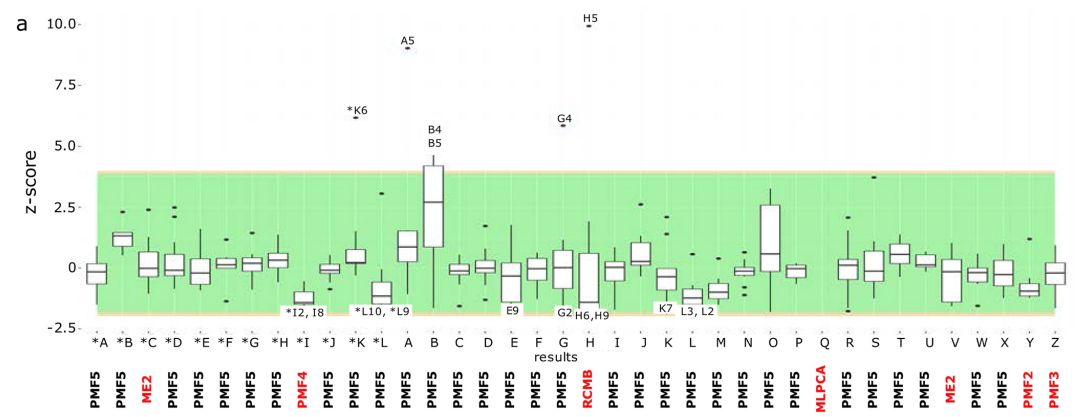
\includegraphics[width=1.0\linewidth]{chapter01/belisEvaluation2020_fig2a.png}
    \caption{Comparabilité des séries temporelles obtenues par les 38 différentes solutions
    sur l'étude de comparaison des modèles sources-récepteurs sur le site de Lens par
    rapport à la moyenne de l'ensemble des différentes études. L'axe X représente chacune des
    solutions des participants, et l'axe Y le z-score, mesure de la similitude des
contributions temporelles. La solution commune IGE-INERIS-EMD est la solution W.\\
Source: \cite{belisEvaluation2020}}%
    \label{fig:chapter01/belisEvaluation2020_fig2a}
\end{figure}

\subsection{Atouts et limitations des différents modèles récepteurs}%
\label{ssub:atouts_et_limitations_des_différents_modèles_récepteurs}

Les 3 types de modèles listés précédemment (CTM, CMB et PMF) ne sont pas les seuls
utilisés, mais représentent néanmoins la très grande majorité des études d'attribution
des sources. Leurs atouts et limitations sont repris dans le
tableau~\ref{tab:comparison_SA} et nous expliquerons dans cette partie plus en avant le
choix pour cette thèse du modèle PMF avec analyse chimique sur filtre.

\begin{table}[!ht]
    \begin{ThreePartTable}
        \centering
        \caption{Forces et limitations des différents modèles d'attribution des sources}
        \label{tab:comparison_SA}
        \footnotesize
        \begin{tabular}{cp{0.43\textwidth}p{0.43\textwidth}}
        \toprule
        Type & Atouts & Limitations \\
        \midrule
        CTM &
        \begin{itemize}[topsep=0pt, left=0pt, label={\unicodesymbols ✔}]
          \item Grande couverture spatiale et temporelle
          \item Comparaison facilité : sources identiques partout\tnote{a}
          \item Prévision à court et long terme
          \item[{\unicodesymbols ~}] Peu de subjectivité\tnote{b}
        \end{itemize}
            &
        \begin{itemize}[topsep=0pt, left=0pt, label={\unicodesymbols ✘}]
          \item Nécessite des cadastres d'émissions
          \item Nécessite un modèle météo
          \item Ne voit que ce qui est donnée des cadastres
          \item Variabilité temporelle des émissions peu robuste
          \item Nombre d'espèces chimiques limités
        \end{itemize}
        \\ \midrule
        CMB & 
        \begin{itemize}[topsep=0pt, left=0pt, label={\unicodesymbols ✔}]
          \item Spécificité du site potentiellement prise en compte
          \item Grand nombre d'espèces pouvant être utilisé
        \end{itemize}
            & 
        \begin{itemize}[topsep=0pt, left=0pt, label={\unicodesymbols ✘}]
          \item Faible représentativité spatiale et temporelle
          \item Prélèvement et analyses couteux (humain et financier)
          \item Profils des sources fixes et connu à l'avance
          \item Nécessite une base de connaissance de profils chimique
          \item Subjectivité de l'expérimentateur
        \end{itemize}
        \\ \midrule
        PMF &
        \begin{itemize}[topsep=0pt, left=0pt, label={\unicodesymbols ✔}]
          \item Pas besoin de connaissance a priori des sources
          \item Spécificités du site prise en compte
        \end{itemize}
            & 
        \begin{itemize}[topsep=0pt, left=0pt, label={\unicodesymbols ✘}]
          \item Faible représentativité spatiale et temporelle
          \item Prélèvement et analyses couteux (humain et financier)
          \item Nécessite des espèces traceuses
          \item Grand nombre d'échantillons requis
          \item Subjectivité de l'expérimentateur
        \end{itemize}
        \\
        PMF-AMS &
        \begin{itemize}[topsep=0pt, left=0pt, label={\unicodesymbols ✔}]
          \item Grande caractérisation de la matière organique
          \item Possibilité de résolution temporelle très fine (mesure on-line)
        \end{itemize}
            & 
        \begin{itemize}[topsep=0pt, left=0pt, label={\unicodesymbols ✘}]
          \item Difficultés d'interprétation
          \item Cible uniquement la matière non réfractaire
          \item Peu utile pour la réglementation
        \end{itemize}
        \\
        PMF-filtre &
        \begin{itemize}[topsep=0pt, left=0pt, label={\unicodesymbols ✔}]
          \item Large gamme de famille d'espèce chimique
          \item Directement applicable pour la régulation
          \item D'autres analyse possible sur le même filtre (potentiel oxydant par
              exemple)
        \end{itemize}
            & 
        % \begin{itemize}[topsep=0pt, left=0pt, label={\unicodesymbols ✘}]
        % \end{itemize}
        \\
        \bottomrule
        \end{tabular}
    \end{ThreePartTable}
\end{table}


\subsubsection{La PMF : modèle théoriquement le moins biaisé par l'information a priori}%
\label{ssub:choix_du_modèle_pmf}

Lorsque l'on s'intéresse à un site particulier, le contexte géographique peut nous donner
des indications sur les sources majoritaires. Seulement, prédéfinir à l'avance les sources
possibles résulte en un biais évident : on ne voit que ce que l'on s'attend à voir.
L'utilisation des CTM ou du CMB ne nous permet donc pas de découvrir de nouvelles sources
locales. Au mieux, le modèle échouera à reproduire les observations, ce qui indiquerait
une source ou un processus manquant.

Au contraire, la PMF étant totalement agnostique aux sources ou processus réels, les
facteurs déterminés reflètent les observations locales sans biais. Ainsi, l'ajout d'une
espèce peut conduire à découvrir et quantifier une nouvelle source d'émission ou processus
atmosphérique, jusqu'alors non prise en compte ou sous-estimée, comme nous le verrons dans
le chapitre~\ref{cha:approfondissement_des_connaissances_des_sources_des_pm}. À noter
également que la réciproque est vraie : la non-prise en compte d'une espèce chimique peut
conduire à ne pas identifier un facteur important, ayant un impact direct sur la
contribution des autres facteurs aux PM.
Toute la difficulté réside dans le choix des ``bonnes espèces'' et en l'interprétation de
ce modèle, fondé sur nos connaissances géochimiques.

\subsubsection{Analyses chimiques ou spectrométrie de masse}%
\label{ssub:analyses_chimiques_ou_spectrometrie_de_masse}

Comme expliqué précédemment, les PM sont composées en grande majorité de matière organique
--tout du moins dans les écosystèmes européens.  Devant la myriade d'espèces chimiques la
constituant, la caractérisation exhaustive de cette matière organique est illusoire.
Pourtant, il est possible de décrire cette matière organique de manière extrêmement
précise par spectrométrie de masse (\textit{aerosol mass spectrometer} (AMS)). On obtient alors des
fragments d'espèces chimiques ionisées, caractérisés par leur ratio masse sur charge ionique
($m/z$ ou Th).

L'avantage principal est la quasi-exhaustivité et la possibilité de
résolution temporelle fine pouvant aller à un échantillon toutes les 2 minutes
\autocite{marmureanuOnline2020}.  Le désavantage majeur est la quantité extrêmement
importante de données générées à analyser. En plus, l'identification des fragments en
facteur PMF est difficilement interprétable en termes de source d'émission. En effet, si
l'on retrouve des facteurs primaires comme l'\textit{hydrocarbon-like organic} (HOA)
pouvant être relié au trafic ou le \textit{biomass burning organic aerosol} (BBOA),
certains, reflétant des processus secondaires, sont plus ``abstraits'' et classés selon leur
degré d'oxygénation : \textit{less-oxidized oxygenated organic aerosol} (LO-OOA) ou
encore \textit{more-oxidized oxygenated organic aerosol} (MO-OOA).
Enfin, l'utilisation de PMF sur données AMS présente aussi la limitation de ne prendre en
compte que la matière non réfractaire. Il est donc difficile voire impossible d'estimer la
contribution des poussières crustales, présentant très peu ou pas de matière organique. De
même, les émissions secondaires du trafic comme l'usure des freins ou des pneus ne peuvent
pas être retrouvées par PMF-AMS.

Les méthodes de PMF-AMS sont cependant récentes et en développement très rapide et ces
dernières années de nouveaux travaux tentent de combiner mesure AMS et mesures chimiques sur
filtre~\autocite{vlachouAdvanced2018,vlachouDevelopment2019}.  Cependant, lorsque l'on
s'intéresse aux sources d'émissions dans une optique réglementaire et non de compréhension
fine des processus secondaires, la PMF avec analyses chimiques sur filtre reste pour
l'instant davantage adaptée que la PMF-AMS.

En effet, les analyses sur filtres permettent l'identification des types d'espèces
chimiques plus larges qu'uniquement la matière organique (ions et métaux notamment).  Le
recul scientifique des analyses chimiques sur filtres est également appréciable pour
déterminer les sources ou processus à l'œuvre.

Enfin, et plus spécifiquement à cette thèse, nous chercherons à analyser d'autres
variables que la chimie (notamment le potentiel oxydant, voir
section~\ref{sec:le_potentiel_oxydant_des_aerosols}) sur les mêmes échantillons que les
mesures de chimie. Cela exclut donc les données AMS on-line et donc la résolution
temporelle fine, réduisant l'intérêt de cette méthode pour cette thèse.

\subsubsection{Nécessité d'inclure des espèces traceuses dans les PMF}%
\label{ssub:nécessité_d_inclure_des_espèces_traceuses}

L'une des limitations des PMF provient de leur sensibilité aux variables d'entrées
utilisées. La détermination de facteur sera grandement facilité par la présence d'une
espèce chimique permettant l'identification précise de ce facteur.
Par exemple, un facteur ``combustion de biomasse'' peut être déterminé avec uniquement des
espèces métaliques et la présence de potassium, mais l'ajout du lévoglucosan --produit de
pyrolyse de la cellulose-- permet une identification beaucoup plus clair et non équivoque
de ce facteur.

L'utilisation d'\textit{espèces traceuses} rend l'identification de facteur plus aisé,
mais permet aussi la détermination de nouvelle source qui aurait été jusqu'alors peu ou
pas visible.
Par exemple, \cite{srivastavaSpeciation2018a} ont pu déterminer des facteurs peu courrant
grâce à l'ajout de certanes espèces organiques traceuses de différents processus :
\textit{fungal spores} (présence de près de \SI{80}{\percent} de l'arabitol et du sorbitol),
\textit{plant debris} (présence d'alcanes impairs), \textit{biogenic SOA}
(présence de produits d'oxydation de l'isoprène (acide $\alpha$-methylglycerique et 2-methylerythritol) et de
l'$\alpha$-pinène (acide hydroxyglutarique)) et \textit{anthropogenic SOA} (présence
d'acenaphthenequinone, de 6H–dibenzo[b,d]pyran-6-one, de 1,8-naphthalique anhydre et de
DHOPA).
De même, l'analyses des HULIS a permis une meilleure déterminantion des facteurs organiques.
\cite{chevrierChauffage2016} a également utilisée des mesures de radiocarbone et la
séparation en carbone \textit{fossil fuel} et \textit{wood burning} provennant de mesure
d'aethalomètre 33, permettant une séparation et une évaluation des
contributions des facteurs plus précise grâce à ces traceurs spécifiques.

Cependant, bien que l'on sait maintenant l'importance de l'ajout de ces espèces dans les
PMF, la généralisation de l'emploi de ces traceurs est limité par le coût analytique
et l'automatisation de certaines de ces mesures.

\section{Vers une mesure unifiée de l'impact sanitaire : le potentiel oxydant}%
\label{sec:le_potentiel_oxydant_des_aerosols}

Devant la grande variété de chimie, forme, taille, etc. des aérosols, il apparaît
compliqué de résumer la toxicité de l'air que l'on respire à la simple concentration
massique en aérosols. En effet, il est évident que respirer un~\si{\ugm} de sable n'aura
pas le même impact sur notre santé qu'un~\si{\ugm} de mercure ou de plomb.  Seulement, la
mesure des concentrations massiques est l'une des plus simples à implémenter en routine et est également
facilement automatisable, permettant ainsi un premier ordre de grandeur de l'exposition
des populations. Aussi, il est important de rappeler que les aérosols n'ont pas qu'un
impact sanitaire, mais également climatique ou environnemental (voir
section~\ref{ssub:impacts_climatiques} et~\ref{ssub:impacts_environnementaux}),
pour lesquels la mesure de la concentration est tout à fait adaptée.

Bien qu'il ne soit pas encore établi de mécanismes clairs entre les PM et leur impact
sanitaire, leur capacité à induire un stress oxydant dans notre corps est une des
hypothèses privilégiées, notamment par leur transport ou induction d'espèces réactives de
l'oxygène (\textit{reactive oxygen species}
(ROS))~\autocite{squadritoQuinoid2001,liParticulate2003a,liUltrafine2003,gonzalez-flechaOxidant2004}.

La présence de ROS dans nos cellules est un phénomène naturel, produit en grande partie
par catabolisme oxydatif et notamment la respiration cellulaire lors du transfert
d'électron depuis le \ce{O2} vers l'accepteur final \ce{H2O}. Lors de ce transfert, il est
possible d'avoir des électrons captés par d'autres espèces chimiques, conduisant à la
formation de l'anion superoxyde \ce{O2^{.-}} ou \ce{HO^{.-}}, entre autres.
En temps normal, les anti-oxydants cellulaires réduisent ces oxydants avant qu'ils ne
puissent avoir des effets délétères sur les chaînes protéiques ou les acides nucléiques.

Seulement, au contact de nos poumons, les PM, oxydantes, interagissent donc avec nos
anti-oxydants naturels~\autocite{kellyProtein2003}, voir traversent la paroi épithéliale
et entrent dans la circulation générale et les cellules internes, comme illustré
figure~\ref{fig:mecanisme_oxydation}.
Dans un premier temps, les défenses anti-oxydantes sont mobilisées, puis si l'oxydation se
poursuit, on a alors une inflammation puis une cytotoxicité~\autocite{baezaPollution2007}.

\begin{figure}[ht]
    \centering
    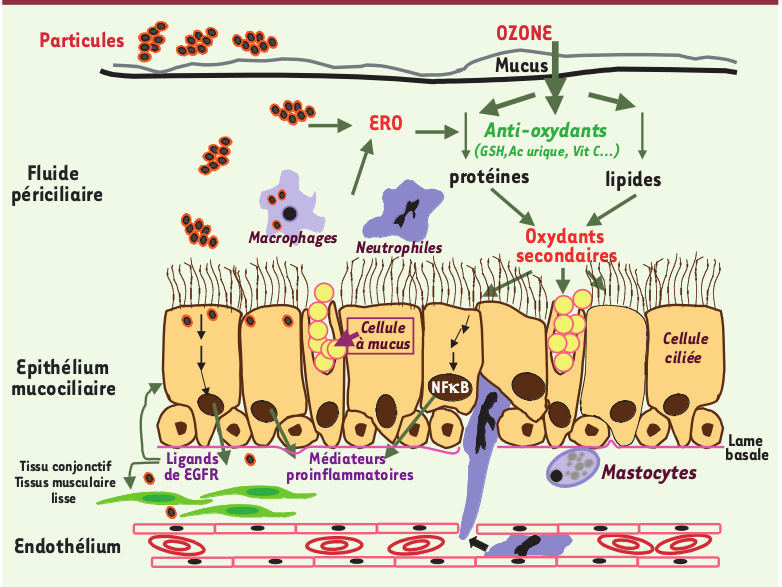
\includegraphics[width=0.8\linewidth]{chapter01/OxydativeMechanism_BaezaMorano2007.png}
    \caption{Mécanismes de toxicité de l’ozone et des particules atmosphériques dans les voies
    aériennes. Crédit : \cite[figure 1]{baezaPollution2007}}%
    \label{fig:mecanisme_oxydation}
\end{figure}

Afin de répondre à cette problématique de métrique sanitaire des PM, il a été proposé
par~\cite{zielinskiModeling1999} et \cite{choRedox2005} une nouvelle mesure, intégratrice
des propriétés physico-chimiques des aérosols, sensée être plus proche des impacts
sanitaires occasionnés par les PM : le \textit{potentiel oxydant} (PO, ou
\textit{oxidative potential} (OP)).  Cette nouvelle mesure tente de quantifier les espèces
réactives de l'oxygène présentes ou induites par les aérosols, en utilisant la mise en
contact des aérosols avec un anti-oxydant.  Le suivi de la cinétique de la réaction permet
ainsi d'estimer la réactivité de l'échantillon, prenant en compte non seulement sa chimie,
mais aussi la taille et forme des particules à travers leurs surfaces de réaction et
également les potentiels ``effet cocktail'' lors de la combinaison de différentes espèces
chimiques.

L'avantage de cette méthode acellulaire réside en son faible coût, mais elle aussi est
non-invasive et implémentable en routine en laboratoire, comparativement aux tests
cellulaires nécessitant des prélèvements de tissu et des analyses des protéines marqueuses de
l'inflammation.  Elle permet également une confrontation facilitée aux autres informations
dont nous disposons sur les PM provenant du même échantillon.

\subsection{Méthodologie de mesure}%
\label{sub:methodologie_de_mesure}

Il n'existe pas à l'heure actuelle de méthodologie standardisée de mesure du potentiel
oxydant. Plusieurs méthodes coexistent et apportent chacune une vision différente du PO.

Il faut noter également que ces méthodes n'ont pas été développées lors de ma thèse mais
s'appuient sur les travaux de \cite{calasPollution2017} et que les échantillons ont été
analysés par les différent·e·s techniciennes et techniciens du plateau analytique
Air-O-Sol de l'IGE.

\subsubsection{Différents agents réactants}%
\label{ssub:differents_agent_reactant}

La mesure du PO se faisant par suivi cinétique de la déplétion d'un anti-oxydant
lorsqu'il est mis au contact des PM, le choix de l'anti-oxydant induit des mesures de PO
différentes. Au cours de cette thèse, 2 mesures différentes sont utilisées conjointement :
le test au dithiothreitol (DTT) et à l'acide ascorbique ou vitamine-A (AA), et sont
explicités dans le chapitre suivant (section~\ref{sub:potentiels_oxydants}).

D'autres méthodes de mesure du PO existent, mais n'ont pas été utilisées au courant de
cette thèse, à savoir :
\begin{description}
    \item[Electron spin résonance ESR] Sensé cibler particulièrement le radical
        \ce{HO^{.}} \autocite{shiHydroxyl2003,shiTemporal2003}
    \item[DCFH] Mesure de la consomation DCFH par suivi de son produit oxydé la DCF, par
        fluorescence \parencite{foucaudMeasurement2007}.
    \item[Mélange d'anti-oxydant (RTLF)] Bien que la plupart du temps testé indépendamment, il est
        possible d'estimer un ``PO moyen'' par la mise en contact de différents
        anti-oxydants simultanément (acide ascorbique, glutation et urée par
        exemple)~\autocite{mudwayDifferences2001,calasComparison2018,gaoCharacterization2020}
    \item[Mesure directe de \ce{HO^{.}}] Développement en cours à l'IGE dans le cadre du
        programme MHYRIAM financé par le LEFE-CHAT.
\end{description}

\subsubsection{Un ``meilleur'' test que les autres ?}%
\label{ssub:un_meilleur_test_que_les_autres_}

Les différents tests de PO ne sont pas sensibles aux mêmes espèces chimiques ni même aux
mêmes conditions physico-chimiques. En effet, l'étude de \cite{kunzliComparison2006} sur
20 sites européens présente des corrélations différentes entre le PO mesuré par ESR, AA ou
GSH au regard de la masse des PM et les métaux les constituant.
Ce résultat a été retrouvé depuis dans de nombreuses études, ainsi que pour le test au DTT et DCFH
également. Par conséquent, cela montre que différents constituants des PM agissent
différemment à travers des mécanismes oxydatifs divers, capturés par certains tests et
non par d'autres.  Il est donc probable que certaines affections sanitaires soient reliées
à un test donné, et d'autres affections à un autre test. En l'absence de travaux plus
approfondis en toxicologie et épidémiologie, il n'est donc pas possible en l'état actuel
des
connaissances de trancher pour ``le meilleur test de PO''.

Par conséquent, les travaux de cette thèse s'emploient à étudier conjointement le PO
mesuré par DTT et par acide ascorbique.


\subsection{Attribution du PO aux sources d'émissions des PM}%
\label{sub:attribution_du_po_aux_sources_d_émissions_des_pm}

Les mesures de PO étant fastidieuses, il a fallu attendre la mise en place de techniques
de semi-automatisation pour obtenir des séries temporelles de mesure de ``longue durée''. Les récents
travaux de \cite{fangSemiautomated2015}, parallèlement aux travaux de
\cite{calasPollution2017}, ont permis ce pas technique, permettant l'analyse accrue de
prélèvements et les premières séries annuelles de mesure des PO, conjointement avec
l'analyse de la chimie des filtres prélevés.

\subsubsection{Mesure directe du PO des espèces chimiques}%
\label{ssub:mesure_directe_du_po}

La famille des quinones est suspectée d'avoir un rôle majeur dans le stress oxydatif.
La mesure du PO de solutions de différentes quinones montre en effet leurs fortes
réactivitées vis-à-vis des différents tests de PO
\parencite{ayresEvaluating2008,charrierDithiothreitol2012,jiangOxidative2016,calasImportance2017,wangRelationship2018}.
Certains métaux, et notamment le cuivre ou le manganese, présentent aussi un potentiel
oxydant important \parencite{charrierDithiothreitol2012,charrierBias2016}.
Cependant, tous les métaux ne réagissent pas de façons similaire et d'autres comme le fer,
le zinc ou le cromium ne présentent pas de réactivité particulière au test du DTT.

Il faut noter également que la consomation d'antioxydant de ces différents composés
n'augmente pas systématiquement linéairement avec la masse
\parencite{ayresEvaluating2008,charrierDithiothreitol2012,calasImportance2017}.
De plus, des effets synergiques sont observés 
\parencite{charrierDithiothreitol2012,charrierHydrogen2014,xiongRethinking2017,samakeUnexpected2017}
où le mélange de deux composés n'est pas nécessairement la somme de l'action des composés
pris individuellement.

Cependant, il n'est pas possible de mesurer l'ensemble des espèces chimiques constituant
les PM. Devant cette foultitude, il paraît donc illusoire de pouvoir attribuer un PO
intrinsèque à chacune des espèces chimique.

\subsubsection{Corrélation PO -- chimie}%
\label{ssub:corrélation_po_chimie}

Afin d'estimer la provenance du PO des particules, les liens entre la chimie PM et les
résultats de PO se sont dans un premier temps focalisés sur la simple corrélation univariée.
Conformément aux mesures directes, le cuivre présente une
forte corrélation avec le \PODTT{} et \POAA, de même que le carbone organique et les HULIS
\parencite{vermaFractionating2015,batesReview2019}.
Seulement, il est aussi mis en évidence une forte corrélation entre le \PODTT{} et le
\NOt, pourtant inerte en termes d'oxydo-réduction.

En effet, une corrélation n'implique pas une causalitéi. Cette corrélation ne résulte donc
que d'une co-correlation entre le \NOt{} d'autres espèces qui, elles, sont, rédox-actives.

L'étude de la corrélation simple permet donc une première estimation des déterminants du
PO, mais se révèle être insufissante.


\subsubsection{Sources de PM et de PO}%
\label{ssub:sources_de_pm_et_de_po}

% En revanche, si l'on bénéficie d'un nombre suffisant d'échantillon, il est alors possible
% d'estimer les sources ou facteurs d'émissions (voir
% section~\ref{sec:source_apportionment_of_pm}). Ce faisant, la vision par ``source'' plutôt
% que par ``espèce'' permet une agrégation de l'information, en regroupant un ensemble
% d'espèce, mesurée ou non, provenant d'une même source d'émission, en une seule variable.
% Ainsi, il est possible d'attribuer un PO à une source donnée, sans pour autant avoir
% besoin de savoir quelles sont les espèces chimiques émises par cette source qui
% contribuent au PO.
Il est aussi possible de chercher à attribuer un PO non pas à une espèce chimique mais à
une source d'émission spécifique.
Cette vision par source présente également l'avantage de pouvoir se traduire plus
simplement en terme de régulation de la qualité de l'air et permet
potentiellement une action politique plus rapide que s'il s'agissait de cibler une espèce
chimique particulière.

\paragraph{Mesures directes à l'émission}%
\label{par:mesures_directes_à_l_émission}

La méthode la plus intuitive de mesure du PO des sources de PM est de faire les analyses
directement à l'émission. Les sources les plus échantillonées sont différentes émissions
liées aux trafic routier \parencite{biswasOxidative2009,parkDifferential2018} ou à l'industrie
\cite{jooPhysicochemical2018}, ainsi que la combustion de biomasse
\parencite{jiangOxidative2016,parkDifferential2018} (voir notamment la revue de \cite{batesReview2019}).
Certaines autres mesures peuvent être effectuées également en chambre de simulation : SOA, spray marin, etc.
\parencite{parkDifferential2018}.

Les sources d'émissions liés aux émissions primaire du trafic semblent avoir un \PODTTm{}
intrinsèque (i.e. par microgramme de PM) du même ordre de grandeur que les émissions de
combustion de biomasse. En revanche, les OAS d'origines biogéniques présentent un \PODTTm{}
plus faible et une variabilité importante.

Il semblerait quand meme tres intéressant de mesurer le PO sur des filtres collectés
directement lors de l'émission pour de nombreux types de sources car c'est en définitive
le type de mesure le plus fiable (mais sans prise en compte de phénomènes secondaires).
De plus, de nombreux secteur d'émissions doivent déjà présenter des prélèvements
caractérisations chimiques (banc d'essai, industrie, etc). 
Il est également probable que de nombreux programmes de caractériation des émissions permettraient
de rassembler le matériel nécessaire à ces mesures de PO, qui ne demandent pas de grandes
surfaces de filtre par rapport aux surfaces prélevées.

Seulement, bien que renseignant sur la potentiel toxicité des sources, ces mesures à
l'émissions ne permette pas directement de quantifier l'exposition des populations, qui
doit également prendre en compte la contribution de chacune des sources aux PM ambiantes.

\paragraph{Études sur sites et en air ambiant}%
\label{par:études_sur_sites_et_en_air_ambiant}

Les premières études de ce type sont celles de
\cite{vermaReactive2014,batesReactive2015,fangOxidative2016}, et utilisent 2 approches
différentes :
\begin{enumerate}
    \item Incorporation de PO comme variable d'entrée d'une étude PMF au même titre qu'une
        autre espèce chimique ;
    \item Analyse de sources via le CMB (sans PO), puis régression linéaire entre les
        sources de PM ainsi déduites et le PO.
\end{enumerate}
Bien que, de façon inhérente aux différences entre PMF et CMB, les sources retrouvées ne
sont pas exactement les mêmes, les auteurs montrent que la combustion de biomasse est la source
principale de \PODTTv, suivie de près par le trafic routier (ensemble des émissions
véhiculaires et de la remise en suspension de poussière de route), puis le sulfate
d'ammonium et enfin un facteur de composés organiques secondaires solubles.
Concernant le \POAAv, \cite{fangOxidative2016} (voir
figure~\ref{fig:chapter01/fangOxidative2016-fig4}) estiment à autour de \SI{45}{\percent} la
contribution des émissions véhiculaires et à environ \SI{50}{\percent} la contribution de
facteur secondaire (organique et inorganique).

\begin{figure}[ht]
    \centering
    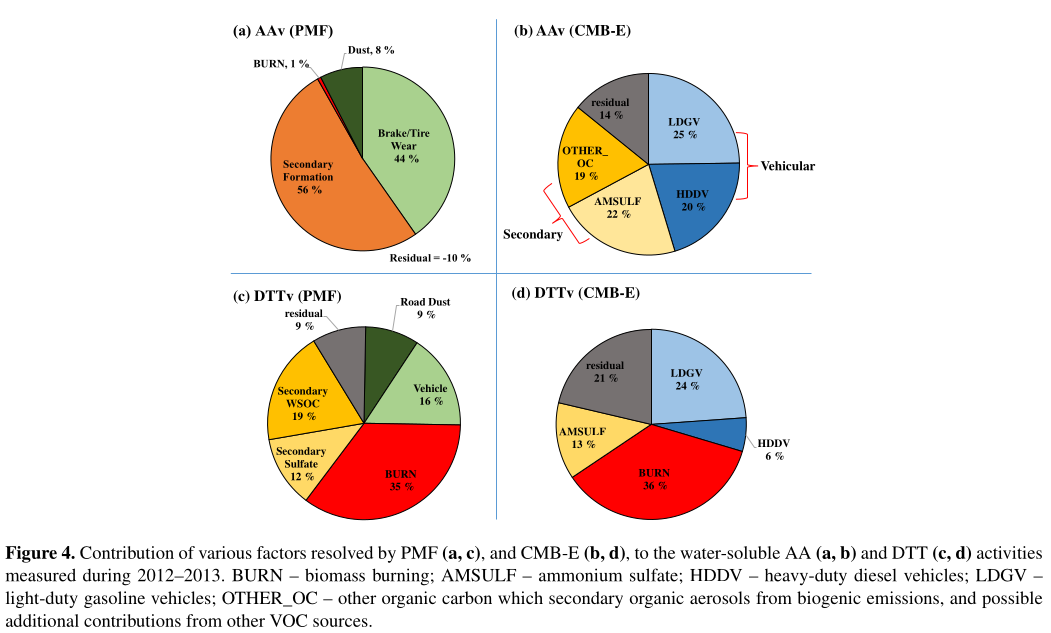
\includegraphics[width=1.0\linewidth]{chapter01/fangOxidative2016-fig4.png}
    \caption{Contribution des sources de PM aux \POAAv{} et \PODTTv{} par l'étude de
    \cite{fangOxidative2016} portant sur un ensemble de 238 échantillons sur 3 sites
        distincts à Atlanta, US, pendant l'année 2012-2013.}%
    \label{fig:chapter01/fangOxidative2016-fig4}
\end{figure}

Lors du commencement de ma thèse, seules ces études étaient, à ma connaissance,
disponibles dans la littérature concernant l'attribution des sources de PM aux potentiels
oxydants.  Depuis, de nouvelles études ont été publiées, et seront discutées dans le
chapitre~\ref{cha:estimation_des_sources_de_PO}.


\section{Objectifs de cette thèse}%
\label{sec:positionnement_de_cette_thèse}

\subsection{Problématique générale}%
\label{sub:problématique_générale}

Ma thèse s'inscrit donc dans cette double problématique de l'identification et de la
quantification des contributions massiques des différentes sources d'émission de PM en air
extérieur, mais aussi de leurs contributions au nouvel indicateur qu'est le potentiel
oxydant.

Premièrement, il s'agit d'améliorer l'outil de déconvolution des sources de PM
\textit{Positive Matrix Factorization}. Cette amélioration ne concernent pas de nouveaux
développements mathématiques de résolution de l'équation de conservation des masses, mais
l'élaboration d'une expertise dans les différentes paramétrisations de ce modèle, dans son
entraînement et dans la critique de ses résultats.
Notamment, la question de la prise en compte ou non des sources majoritaires de PM dans
les solutions PMF se posera dans le
chapitre~\ref{cha:approfondissement_des_connaissances_des_sources_des_pm}, à travers
l'implémentation de nouveaux traceurs chimiques ou isotopiques.
Également, les incertitudes des solutions PMF ne sont que rarement explicitées alors
mêmes que c'est une question centrale qui intéressent d'autant plus les décideurs publics.
Mes travaux s'appliquerons donc à systématiquement quantifier les incertitudes des
contributions des sources de \PMdix{} aux espèces mesurées.
Aussi, afin de pouvoir généraliser à large échelle spatiale des résultats issus d'études
PMF sur différents sites, une méthodologie harmonisée doit être employée (mêmes espèces
chimiques, mêmes contraintes…), mais la similitude géochimique des différents facteurs
doit également être objectivée.

Enfin, l'estimation des sources majoritaires du potentiel oxydant des PM se doit d'être
quantifiée, aussi bien en termes de \POm{} --PO par microgramme, reflétant la toxicité de
la source-- que de \POv{} --PO par mètre cube d'air, reflétant l'exposition à cette
source.  Aussi, les différences de contributions des sources entre concentration massique
et potentiel oxydant, qui ont commencés à être mise en évidence par les études
antérieures, manque de généralisation spatiale. Les études précédentes ne couvrant que peu
de sites de prélèvements différents et présentant une étendue temporelle limitée.


\subsection{Questionnement et plan de la thèse}%
\label{sub:plan_de_la_thèse}

Ainsi, mes recherches tenteront de répondre aux questions suivantes :

\begin{itemize}
    \item Comment obtenir des contributions et profils de sources reflétant au mieux les
        processus d'émissions et de transformation dans l'atmosphère ?
        (Chapitre~\ref{cha:approfondissement_des_connaissances_des_sources_des_pm})
    \item Est-il possible de diminuer la subjectivité de l'expérimentateur dans ces
        études d'attribution des sources ?
        (Chapitre~\ref{cha:approfondissement_des_connaissances_des_sources_des_pm})
    \item Comment comparer efficacement 2 profils attribués à la même source, à
        différents sites de prélèvement et différentes années de mesure ?
        (Chapitre~\ref{cha:approfondissement_des_connaissances_des_sources_des_pm})
    \item Comment remonter à la contribution des sources de PO une fois les sources
        d'émissions de PM identifiées ?
        (Chapitre~\ref{cha:estimation_des_sources_de_PO})
    \item Les sources contribuant au potentiel oxydant sont-elles les mêmes que celles
        contribuant à la masse des PM ?
        (Chapitre~\ref{cha:estimation_des_sources_de_PO})
    \item Est-ce que les valeurs PO des sources des PM sont les mêmes à large échelle spatiale ou
        sont-elles dépendantes du lieu considéré ?
        (Chapitre~\ref{cha:estimation_des_sources_de_PO})
    \item Est-il possible, à terme, d'obtenir une prévision du PO intégré à la prévision
        de la qualité de l'air, complémentairement à la concentration massique ?
        (Chapitre~\ref{cha:estimation_des_sources_de_PO} et~\ref{cha:travaux_futur})
\end{itemize}

Ces différentes questions seront abordées entre autres avec la présentation des résultats de
recherches déjà publiés dans 7 articles scientifiques auxquels j'ai contribué (dont 2 
en premier auteur) ainsi qu'avec des travaux en cours de publication (6, dont 2 en premier auteur).
La liste complète de ces travaux est fournie en annexe~\ref{annexe:CV} et s'appuie sur un
grand nombre de programmes de recherche
(voir~\ref{annexe:programmes_ayant_financés_la_thèses}) et des travaux que j'ai encadré
(voir~\ref{annexe:CV}). Les articles en premier auteur sont reproduits in extenso.
